% PowerLab user manual.
% Build: python tools/make_manual.py --pdf   (or: latexmk -pdf -outdir=build manual.tex)
% The tables in generated/ and the screenshots in figures/ come from
% tools/make_manual.py; do not edit them by hand.
\documentclass[11pt, a4paper, parskip=half, toc=bibliographynumbered, open=any,
               headings=standardclasses, numbers=noenddot]{scrreprt}

% --------------------------------------------------------------------------
% Fonts and language
% --------------------------------------------------------------------------
\usepackage[T1]{fontenc}
\usepackage[utf8]{inputenc}
\usepackage[english]{babel}
\usepackage{libertinus}
\usepackage[scaled=0.92]{inconsolata}
\usepackage{microtype}

% --------------------------------------------------------------------------
% Layout
% --------------------------------------------------------------------------
\usepackage[a4paper, top=2.6cm, bottom=2.8cm, left=2.5cm, right=2.5cm,
            headheight=15pt]{geometry}
\usepackage[automark, headsepline]{scrlayer-scrpage}
\pagestyle{scrheadings}
\clearpairofpagestyles
\ihead{\small\headmark}
\ohead{\small PowerLab 1.0 User Manual}
\cfoot*{\small\pagemark}
\setcounter{tocdepth}{1}
\setcounter{secnumdepth}{2}

% --------------------------------------------------------------------------
% Packages
% --------------------------------------------------------------------------
\usepackage{amsmath, amssymb, mathtools}
\usepackage{graphicx}
\usepackage{xcolor}
\usepackage{booktabs}
\usepackage{array}
\usepackage{tabularx}
\usepackage{xltabular}
\usepackage{enumitem}
\usepackage{caption}
\usepackage{float}
\usepackage{needspace}
\usepackage{tikz}
\usepackage{listings}
\usepackage[most]{tcolorbox}
\usepackage[os=win]{menukeys}
\usepackage{siunitx}
\sisetup{group-separator={,}, group-minimum-digits=4}
\usepackage[hidelinks, pdfusetitle]{hyperref}
\usepackage[capitalise, noabbrev]{cleveref}

% --------------------------------------------------------------------------
% Colours (the application's palette)
% --------------------------------------------------------------------------
\definecolor{plblue}{HTML}{1F5FA8}
\definecolor{plink}{HTML}{141719}
\definecolor{plgrey}{HTML}{5B666E}
\definecolor{plpaper}{HTML}{F4F6F7}
\definecolor{plline}{HTML}{CFD6DB}
\definecolor{plgreen}{HTML}{1E7A4E}
\definecolor{plamber}{HTML}{B9770E}
\definecolor{plred}{HTML}{B42318}

\addtokomafont{disposition}{\color{plblue}}
\addtokomafont{chapter}{\Huge}
\setkomafont{captionlabel}{\sffamily\bfseries\small}
\setkomafont{caption}{\small}
\captionsetup{margin=10pt}
\hypersetup{colorlinks=true, linkcolor=plblue, urlcolor=plblue, citecolor=plblue}

\setlist{itemsep=2pt, topsep=4pt}
\setlist[description]{font=\sffamily\bfseries\color{plink}, leftmargin=1.5em}

% --------------------------------------------------------------------------
% Markup for the manual
% --------------------------------------------------------------------------
\newcommand{\app}{PowerLab}
\newcommand{\gui}[1]{\textsf{\textbf{#1}}}            % a label on the screen
\newcommand{\code}[1]{\texttt{#1}}                    % a value, field or option name
\newcommand{\file}[1]{\texttt{#1}}                    % a file or folder
\newcommand{\cli}[1]{\texttt{#1}}                     % something typed in a terminal
\newcommand{\pu}{\,\mathrm{pu}}
\renewcommand{\Re}{\operatorname{Re}}
\renewcommand{\Im}{\operatorname{Im}}
\newcommand{\conj}[1]{{#1}^{*}}
\newcommand{\figwidth}{\linewidth}

\renewmenumacro{\menu}[>]{roundedmenus}
\renewmenumacro{\keys}[+]{shadowedroundedkeys}

\tcbuselibrary{skins, breakable}
\newtcolorbox{tip}{enhanced, breakable, colback=plblue!5, colframe=plblue!55,
  boxrule=0.5pt, arc=2pt, left=8pt, right=8pt, top=5pt, bottom=5pt,
  fonttitle=\sffamily\bfseries\small, title=Tip, coltitle=white}
\newtcolorbox{note}{enhanced, breakable, colback=plpaper, colframe=plline!80!black,
  boxrule=0.5pt, arc=2pt, left=8pt, right=8pt, top=5pt, bottom=5pt,
  fonttitle=\sffamily\bfseries\small, title=Note, coltitle=white,
  colbacktitle=plgrey}
\newtcolorbox{caution}{enhanced, breakable, colback=plred!4, colframe=plred!60,
  boxrule=0.5pt, arc=2pt, left=8pt, right=8pt, top=5pt, bottom=5pt,
  fonttitle=\sffamily\bfseries\small, title=Caution, coltitle=white}
\tcbuselibrary{listings}
\newtcblisting{terminal}{enhanced, breakable, listing only, colback=plink!3,
  colframe=plink!25, boxrule=0.4pt, arc=2pt, left=6pt, right=6pt, top=1pt, bottom=1pt,
  listing options={basicstyle=\ttfamily\small, columns=fullflexible, keepspaces=true,
    breaklines=true, breakindent=2em, upquote=true, showstringspaces=false}}

% A step-by-step procedure
\newlist{steps}{enumerate}{1}
\setlist[steps]{label=\textsf{\textbf{\arabic*.}}, leftmargin=2em, itemsep=3pt}

% A screenshot with a thin frame
\newcommand{\shot}[2][\linewidth]{%
  \begingroup\setlength{\fboxsep}{0pt}\setlength{\fboxrule}{0.4pt}%
  \fcolorbox{plline}{white}{\includegraphics[width=\dimexpr#1-2\fboxrule\relax]{figures/#2}}%
  \endgroup}

% Numbered callout on the window overview (positions from tools/make_manual.py)
\newcommand{\windowcallout}[3]{%
  \node[circle, fill=plblue, text=white, font=\sffamily\bfseries\small,
        inner sep=1.6pt, minimum size=15pt, draw=white, line width=0.8pt]
        at (#1, #2) {#3};}

% The same numbers in running text
\DeclareRobustCommand*{\calloutnum}[1]{\tikz[baseline=(n.base)]\node[circle, fill=plblue,
  text=white, font=\sffamily\bfseries\scriptsize, inner sep=1pt, minimum size=12pt](n){#1};}

% Generated reference tables
\newenvironment{fieldtable}{%
  \small\renewcommand{\arraystretch}{1.25}%
  \xltabular{\linewidth}{@{}>{\raggedright\arraybackslash}p{3.3cm}%
                            >{\raggedright\arraybackslash}p{1.25cm}%
                            >{\raggedright\arraybackslash}p{2.35cm}%
                            >{\raggedright\arraybackslash}X@{}}
  \toprule
  \sffamily\bfseries Field & \sffamily\bfseries Unit & \sffamily\bfseries Default
    & \sffamily\bfseries Meaning \\ \midrule \endfirsthead
  \toprule
  \sffamily\bfseries Field & \sffamily\bfseries Unit & \sffamily\bfseries Default
    & \sffamily\bfseries Meaning \\ \midrule \endhead
  \bottomrule \endfoot}%
  {\endxltabular}
\newcommand{\fieldgroup}[1]{%
  \multicolumn{4}{@{}l}{\sffamily\bfseries\color{plblue}\footnotesize\MakeUppercase{#1}} \\}

\newenvironment{optiontable}{%
  \small\renewcommand{\arraystretch}{1.25}%
  \xltabular{\linewidth}{@{}>{\raggedright\arraybackslash}p{4.2cm}%
                            >{\raggedright\arraybackslash}p{1.9cm}%
                            >{\raggedright\arraybackslash}X@{}}
  \toprule
  \sffamily\bfseries Option & \sffamily\bfseries Kind & \sffamily\bfseries Meaning
    \\ \midrule \endfirsthead
  \toprule
  \sffamily\bfseries Option & \sffamily\bfseries Kind & \sffamily\bfseries Meaning
    \\ \midrule \endhead
  \bottomrule \endfoot}%
  {\endxltabular}

% A table the manual writes by hand
\newenvironment{reftable}[1]{%
  \small\renewcommand{\arraystretch}{1.2}%
  \xltabular{\linewidth}{#1}}{\endxltabular}

% Component heading with its palette icon
\newcommand{\componentsection}[3]{%
  \section[#1]{\raisebox{-0.28\height}{\includegraphics[height=1.35em]{figures/icon-#2}}%
    \hspace{0.45em}#1}\label{sec:component-#2}%
  \noindent\textit{#3}\par}

\title{\app\ 1.0\\[0.3em]\Large User Manual}
\author{}
\date{}

\begin{document}

% --------------------------------------------------------------------------
% Title page
% --------------------------------------------------------------------------
\begin{titlepage}
  \newgeometry{top=3cm, bottom=2.5cm, left=2.5cm, right=2.5cm}
  \color{plink}
  {\sffamily\bfseries\color{plblue}\fontsize{42}{46}\selectfont \app\par}
  \vspace{0.4cm}
  {\sffamily\Large Interactive single-line diagrams and power system analysis\par}
  \vspace{0.25cm}
  {\sffamily\large\color{plgrey} User Manual\quad$\cdot$\quad Version 1.0.0\par}
  \vspace{1.4cm}
  \noindent\shot[0.97\linewidth]{diagram-lf.png}
  \par\vspace{0.3cm}
  {\small\color{plgrey}\sffamily The Newton--Raphson load flow of the EG2100 Assignment LF
  network, as \app\ annotates and exports it.\par}
  \vfill
  \begin{minipage}[t]{0.58\linewidth}\small\sffamily\color{plgrey}
    \app\ grew out of the course EG2100 Power System Analysis (KTH). It draws a
    network on a canvas and solves, in per unit and with every number traceable:
    two-port matrices, equivalent impedances, bus voltages, the admittance matrices
    of the three sequence networks, Thevenin equivalents, short circuits of every
    type, unbalanced loads and the Newton--Raphson load flow.
  \end{minipage}\hfill
  \begin{minipage}[t]{0.38\linewidth}\raggedleft\small\sffamily\color{plgrey}
    \href{https://github.com/akamaxe/powerlab}{github.com/akamaxe/powerlab}\\[0.3em]
    \today
  \end{minipage}
  \restoregeometry
\end{titlepage}

\tableofcontents

\chapter{Introduction}\label{ch:introduction}

\app\ is an interactive single-line diagram editor with a power system analysis engine
behind it. You draw a network on a canvas, much as in DIgSILENT PowerFactory, PSS/E or
ETAP. \app\ converts it to per unit and runs the studies a power system analysis course
asks for, with the results printed the way the course prints them. It started from the
KTH course \emph{EG2100 Power System Analysis}. Version~1.0 solves all four course
assignments (S1, S2, S3 and LF) and reproduces their reference solutions digit by digit.

\section{What \app\ does}

\begin{description}
  \item[Draw] buses, external grids, generators, two-winding transformers, PI-model lines
    and cables, loads, shunt capacitors and reactors, static var compensators and raw
    impedances. Wires route themselves at right angles. Busbars resize, labels stay
    upright, and every edit can be undone (\cref{ch:drawing,ch:components}).
  \item[Parametrise] any numeric field with an expression over project variables, such as
    \code{(217 + A)/1000}. Change \code{A} and the whole network is re-evaluated
    (\cref{ch:parameters}).
  \item[Organise] the work in \emph{study cases}. A case is a study, its options and,
    optionally, a variant of the network: elements taken out of service and fields
    overridden by an expression. The drawn network is never changed (\cref{ch:cases}).
  \item[Analyse] with eleven studies (\cref{ch:studies}):
    \begin{itemize}
      \item the per-unit model and the sequence model;
      \item two-port (ABCD) matrices, equivalent impedances and linear bus voltages;
      \item the positive-, negative- and zero-sequence admittance matrices;
      \item Thevenin equivalents in all three sequences;
      \item three-phase, single line-to-ground, line-to-line and double line-to-ground
        faults through fault and ground impedances;
      \item unbalanced loads;
      \item the Newton--Raphson load flow, with its iteration log and Jacobian.
    \end{itemize}
  \item[Read] each result in its own tab: a headline, warnings and tables formatted like
    MATLAB's \code{format short}. Annotate the diagram with any result and colour it by
    voltage level or bus voltage (\cref{ch:results}).
  \item[Edit in bulk] every element of a type in the data manager, a spreadsheet-like
    table (\cref{ch:data-manager}).
  \item[Export] results as text, CSV, LaTeX tables or JSON, the diagram as PNG, SVG or
    PDF, and matrices as MATLAB literals that keep every digit (\cref{ch:export}).
  \item[Automate] from a terminal with \file{run\_headless.py}, which runs a project's
    cases, sets variables and exports what it ran (\cref{ch:console}).
\end{description}

\section{Principles}

Four ideas run through the program, and they explain most of its behaviour.

\begin{description}
  \item[Glass box.] Every number can be traced. The per-unit table shows each component's
    conversion with its base factor. The admittance, impedance and Jacobian matrices are
    printed with row and column labels, and the load flow logs every iteration.
  \item[Verified.] Each study checks itself by a second, independent method. The Thevenin
    impedance is computed from the impedance matrix and again by Kron reduction. The
    two-port matrix comes from the element cascade and from the Y-bus. The load flow
    closes the power balance. The cross-check residuals are part of the results.
  \item[Parametric.] Variables, expressions and study cases let one project hold every
    variant of a problem, and re-evaluate it when a parameter changes.
  \item[Course-grade presentation.] Impedance and complex power are printed in rectangular
    form, voltage and current in polar form with the angle in degrees, and matrices with
    MATLAB's common factor (\code{1.0e+02 *}).
\end{description}

\section{About this manual}

\Cref{ch:getting-started} gets you from installation to a first solved network in a few
minutes. \Cref{ch:window,ch:drawing} explain the window and the editor, and
\cref{ch:components} is the reference for every component and field. Then come per-unit
bases (\cref{ch:bases}), parametric variables (\cref{ch:parameters}) and study cases
(\cref{ch:cases}). \Cref{ch:studies} explains each study: what it computes, its options
and its output. \Cref{ch:results,ch:data-manager,ch:export,ch:console} cover reading,
editing in bulk, exporting and the command line. \Cref{ch:assignments} walks through the
four EG2100 assignments task by task, \cref{ch:files} describes the project file, and
\cref{ch:troubleshooting} lists the messages you may meet and what to do about them. The
appendices collect the model equations, the keyboard shortcuts and how the program is
verified.

Conventions used in this manual:

\begin{itemize}
  \item Labels on the screen are set like \gui{Properties}. Menu paths look like
    \menu{File > Export results...}, and keys like \keys{\ctrl + S}.
  \item Field names, option names and values are set like \code{p\_mw} or
    \code{constant\_power}. These are the names that bindings, overrides and the project
    file use.
  \item File names look like \file{examples/lf\_220kv.psn}, and commands typed in a
    terminal like \cli{python run\_gui.py}.
  \item The reference tables of \cref{ch:components,ch:studies} are generated from the
    program's own field definitions, so they always match the version this manual
    describes.
\end{itemize}

\section{Scope of version 1.0}

\app~1.0 models the balanced three-phase network in per unit, with symmetrical components
for unbalanced conditions. It does not yet model breakers and switches as components,
three-winding transformers, off-nominal taps or phase shifters, transformer phase shifts
in the sequence networks, IEC~60909 short circuits (voltage factors), a distributed slack,
or dynamics. \Cref{sec:limitations} lists the limitations, and \file{docs/ROADMAP.md} in
the repository lists what comes next.

\chapter{Getting started}\label{ch:getting-started}

\section{Requirements and installation}

\app\ is a Python program. It needs:

\begin{itemize}
  \item Python 3.10 or later (it is tested with the Anaconda distribution, Python 3.12);
  \item \textbf{PySide6} (Qt~6) for the window;
  \item \textbf{numpy}, \textbf{scipy} and \textbf{networkx} for the engine.
\end{itemize}

Anaconda already ships numpy, scipy and networkx. PySide6 comes from pip:

\begin{terminal}
pip install PySide6 numpy scipy networkx
\end{terminal}

There is nothing to build. Get the repository (\cli{git clone} or a downloaded archive),
open a terminal in its root folder, the one that holds \file{run\_gui.py}, and start the
program from there. The console tools of \cref{ch:console} do not need PySide6.

\begin{note}
On Windows with Anaconda, Qt~6 can fail to load with \emph{``the specified procedure
could not be found''}, because Anaconda ships its own ICU library and that one shadows the
library Qt expects. \app\ works around it: the package \code{psa.gui} preloads the system
ICU when it is imported. \file{run\_gui.py} already imports it first. If you write a
script that uses PySide6 together with \app, import \code{psa.gui} before anything else
from PySide6.
\end{note}

\section{Starting the program}

\begin{terminal}
python run_gui.py                   # an empty project
python run_gui.py --example         # the validated Assignment S1 network (A = 80)
python run_gui.py my_network.psn    # open a project
\end{terminal}

\begin{itemize}
  \item \cli{--example} opens \file{examples/s1\_a80.psn} as an \emph{untitled copy}:
    \keys{\ctrl + S} asks where to save it and never overwrites the example.
    \menu{File > Load Assignment S1 example} does the same from inside the program.
  \item If the file named on the command line does not exist or is damaged, \app\ still
    starts, with an empty project, and tells you why it could not open the file.
  \item If the project links a variable script (\cref{sec:script}), \app\ asks before it
    runs the script. Opening a file never executes code by itself.
  \item The list of recent files and the window layout are stored per user. On Windows
    they live in the registry, under \file{HKCU\textbackslash Software\textbackslash
    PowerLab\textbackslash PowerLab}.
\end{itemize}

\section{A first session in five minutes}\label{sec:first-session}

This walk-through uses the load flow example that comes with \app, so you can see the
whole cycle before drawing anything yourself.

\begin{steps}
  \item Start \app\ and open \file{examples/lf\_220kv.psn} with \menu{File > Open...}
    (\keys{\ctrl + O}). The canvas shows eight 220~kV buses. The slack generator G1 is at
    bus~1, an SVC at bus~3, generator G7 at bus~7, constant-power loads at buses 4, 6 and
    8, and a capacitor at bus~5.
  \item Look at the \gui{Study cases} panel on the right. The project holds three cases:
    \gui{LFa-LFc) Load flow}, \gui{LFd)}, which raises one load by 10\,\%, and the
    \gui{LF variant)} with the shunt rated as a susceptance.
  \item Press \keys{F5} (\menu{Calculate > Run all cases}). Each case gets a tab in the
    \gui{Results} panel at the bottom, and the diagram is annotated with the first one.
    Every bus shows its voltage, angle and type, every line its power flow and losses,
    and every generator its $P$ and $Q$.
  \item Read the headline of the first tab: \emph{Converged in 4 iterations. P\_loss =
    22.1658 MW}. Scroll down for the bus table, the generation table, the branch flows,
    the power balance, the iteration log and the Jacobian.
  \item Click the \gui{LFd)} tab. The annotations switch to that case: the losses rise to
    24.3993~MW.
  \item In the \gui{Variables} panel, double-click the \gui{Expression} cell of \code{A},
    change \code{80.0} to \code{0} and press \keys{Enter}. The loads that depend on \code{A} change. The result
    tabs are marked with an asterisk, and a banner over the canvas says that the results
    are out of date. Press \keys{F5} again: the losses are now 26.4240~MW, the answer
    printed in the assignment for $A=0$.
  \item Try \menu{View > Colour by > Voltage result} to colour each bus by its voltage
    band, and \menu{File > Export diagram...} to save the annotated drawing as a PNG, SVG
    or PDF file.
\end{steps}

\begin{tip}
\menu{Edit > Undo} (\keys{\ctrl + Z}) takes back the change of \code{A} too. Undo covers
every change to the network, the layout, the variables, the bases and the study cases.
\end{tip}

\section{The example projects}

The folder \file{examples/} holds one project per assignment. All of them are parametric
in the variable \code{A}, the student's A-number, and are set to $A=80$. Set it to $0$ to
reproduce the answers printed in the assignment statements.

\begin{reftable}{@{}>{\raggedright\arraybackslash}p{3.8cm}X@{}}
\toprule
\sffamily\bfseries File & \sffamily\bfseries Contents \\ \midrule
\file{s1\_a80.psn} & Assignment S1: a factory fed from a 40~kV grid through two
  transformers and two cable sections. Cases for the per-unit model, S1a, S1b and S1c. \\
\file{s2\_grid.psn} & Assignment S2 and S3a--S3c: the meshed 40~kV grid fed from 70~kV,
  with its zero-sequence data. \\
\file{grid\_industry.psn} & The S2 grid with the S1 industry connected at bus~7: cases
  S2a--S2d and S3a--S3e. \\
\file{lf\_220kv.psn} & Assignment LF: the eight-bus 220~kV network for the load flow,
  with cases LFa--LFd and the constant-B variant. \\
\bottomrule
\end{reftable}

\Cref{ch:assignments} walks through every task of these projects, with the case that
answers it and the expected numbers.

\chapter{The main window}\label{ch:window}

\begin{figure}[H]
  \centering
  \begin{tikzpicture}
    \node[anchor=south west, inner sep=0] (img)
      {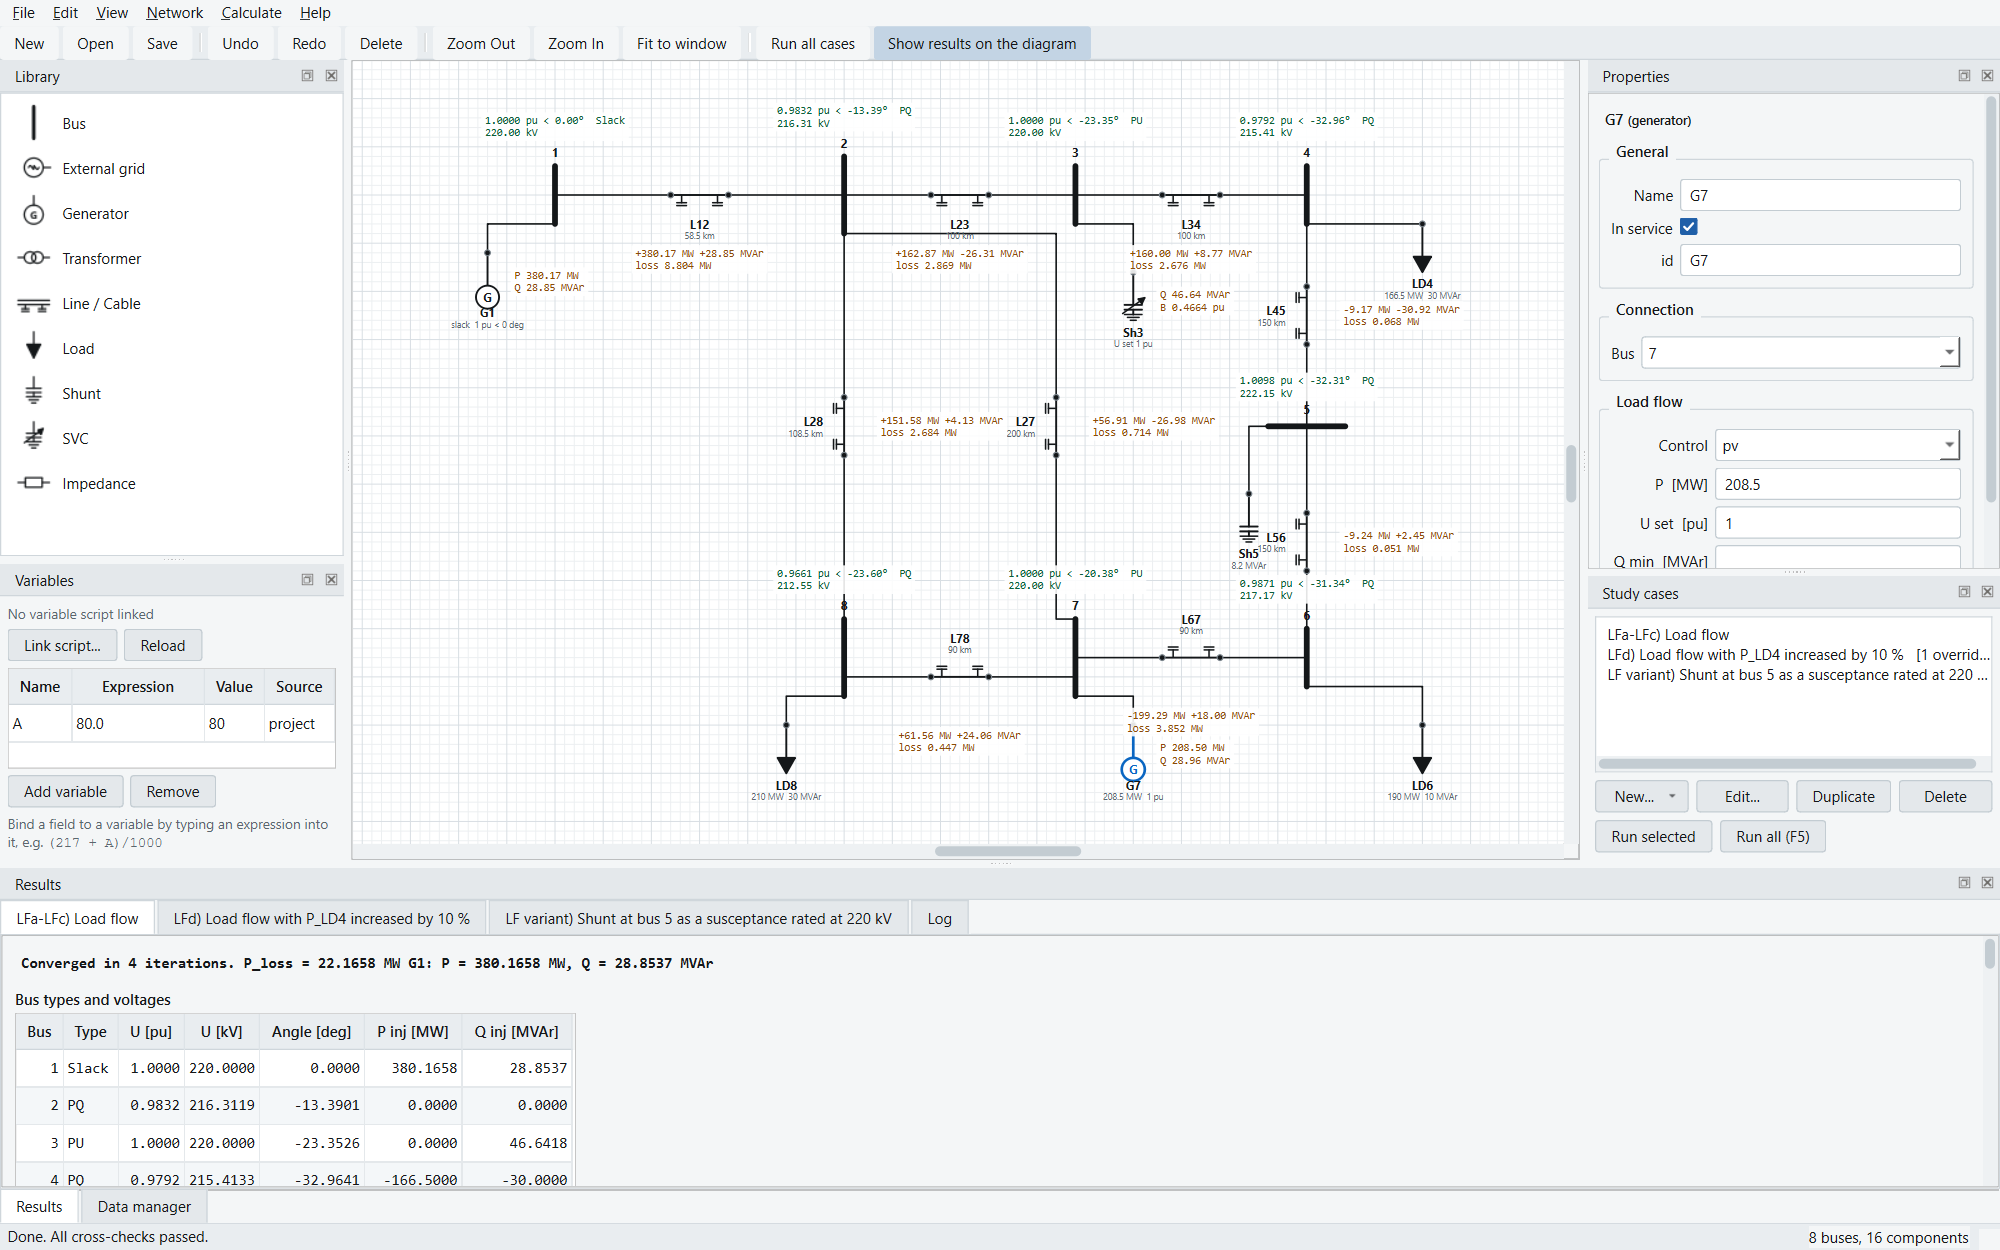
\includegraphics[width=\linewidth]{figures/window-overview.png}};
    \begin{scope}[x={(img.south east)}, y={(img.north west)}]
      % Generated by tools/make_manual.py: callout positions on window-overview.png.
\windowcallout{0.3300}{0.9900}{1}% menubar
\windowcallout{0.6200}{0.9650}{2}% toolbar
\windowcallout{0.1066}{0.9400}{3}% library
\windowcallout{0.1066}{0.5370}{4}% variables
\windowcallout{0.2002}{0.9300}{5}% canvas
\windowcallout{0.9072}{0.9400}{6}% properties
\windowcallout{0.9072}{0.5270}{7}% cases
\windowcallout{0.2000}{0.2940}{8}% results
\windowcallout{0.5000}{0.0120}{9}% status

    \end{scope}
  \end{tikzpicture}
  \caption{The main window with the load flow example after \keys{F5}. The numbers
    match the list below.}\label{fig:window}
\end{figure}

\begin{enumerate}[label=\calloutnum{\arabic*}, leftmargin=2.2em]
  \item \textbf{Menu bar}: \gui{File}, \gui{Edit}, \gui{View}, \gui{Network},
    \gui{Calculate} and \gui{Help} (\cref{sec:menus}).
  \item \textbf{Toolbar}: the most used commands (\cref{sec:toolbar}).
  \item \textbf{Library}: the component palette. Click an entry and then the canvas to
    place it, or drag it onto the canvas (\cref{sec:placing}).
  \item \textbf{Variables}: the project variables, and those read from a linked script
    (\cref{ch:parameters}).
  \item \textbf{Canvas}: the single-line diagram. With results shown, it carries their
    annotations (\cref{sec:annotations}).
  \item \textbf{Properties}: a form for the selected element or elements, generated from
    their fields (\cref{sec:properties}).
  \item \textbf{Study cases}: the cases \keys{F5} runs, with buttons to create, edit,
    duplicate, delete and run them (\cref{ch:cases}).
  \item \textbf{Results} and \textbf{Data manager}: two tabs of one panel. The first holds
    a tab per study result plus a \gui{Log} (\cref{ch:results}), the second the component
    tables (\cref{ch:data-manager}).
  \item \textbf{Status bar}: messages on the left, and the number of buses and components
    on the right.
\end{enumerate}

The panels are dock widgets. Drag a panel by its title bar to move it, to stack it with
another panel as a tab, or to float it as a separate window. Close one with the
\gui{\texttimes} button on its title bar, and bring it back from the \gui{View} menu.
\app\ remembers the layout and the window size between sessions. A layout saved by an
older version that lacked one of today's panels is ignored, and the default layout comes
back.

\section{Menus}\label{sec:menus}

\subsection{File}

\begin{reftable}{@{}>{\raggedright\arraybackslash}p{4.3cm}>{\raggedright\arraybackslash}p{2.6cm}X@{}}
\toprule
\sffamily\bfseries Entry & \sffamily\bfseries Shortcut & \sffamily\bfseries What it does \\ \midrule
\gui{New} & \keys{\ctrl + N} & An empty project. Asks first if the current one has unsaved changes. \\
\gui{Open...} & \keys{\ctrl + O} & Open a \file{.psn} project. \\
\gui{Open recent} & & The last projects opened. \\
\gui{Load Assignment S1 example} & & The S1 network as an untitled copy. \\
\gui{Save} & \keys{\ctrl + S} & Save the project; an untitled one asks for a name. \\
\gui{Save As...} & \keys{\ctrl + \shift + S} & Save under another name. \\
\gui{Export results...} & \keys{\ctrl + E} & Write the last run's results as text, CSV, LaTeX or JSON (\cref{sec:export-results}). \\
\gui{Export diagram...} & \keys{\ctrl + \shift + E} & Save the diagram as PNG, SVG or PDF (\cref{sec:export-diagram}). \\
\gui{Exit} & \keys{\ctrl + Q} & Close \app; asks to save unsaved changes. \\
\bottomrule
\end{reftable}

\subsection{Edit}

\begin{reftable}{@{}>{\raggedright\arraybackslash}p{4.3cm}>{\raggedright\arraybackslash}p{2.6cm}X@{}}
\toprule
\sffamily\bfseries Entry & \sffamily\bfseries Shortcut & \sffamily\bfseries What it does \\ \midrule
\gui{Undo}, \gui{Redo} & \keys{\ctrl + Z}, \keys{\ctrl + Y} & Undo or redo the last change; the entry names it. \\
\gui{Cut}, \gui{Copy}, \gui{Paste} & \keys{\ctrl + X}, \keys{\ctrl + C}, \keys{\ctrl + V} & The clipboard, for elements on the canvas (\cref{sec:clipboard}). \\
\gui{Duplicate} & \keys{\ctrl + D} & Copy and paste the selection in one step. \\
\gui{Delete} & \keys{Del} & Delete the selection (\cref{sec:deleting}). \\
\gui{Select All} & \keys{\ctrl + A} & Select every element. \\
\gui{Find element...} & \keys{\ctrl + F} & Select an element by name or id and centre the diagram on it (\cref{sec:find}). \\
\gui{Rotate 90 deg} & \keys{\ctrl + \Alt + R} & Rotate the selected symbols. \\
\gui{Flip bus orientation} & \keys{\ctrl + \Alt + O} & Switch the selected buses between vertical and horizontal. \\
\bottomrule
\end{reftable}

The clipboard shortcuts act on the canvas only when it has the keyboard focus, so that
\keys{\ctrl + C} in a result table copies the table and \keys{\ctrl + V} in a field pastes
text.

\subsection{View}

\begin{reftable}{@{}>{\raggedright\arraybackslash}p{4.3cm}>{\raggedright\arraybackslash}p{2.6cm}X@{}}
\toprule
\sffamily\bfseries Entry & \sffamily\bfseries Shortcut & \sffamily\bfseries What it does \\ \midrule
\gui{Zoom In}, \gui{Zoom Out} & \keys{\ctrl + +}, \keys{\ctrl + -} & Zoom the canvas. \keys{\ctrl} + mouse wheel zooms around the cursor. \\
\gui{Fit to window} & \keys{\ctrl + 0} & Show the whole diagram. \\
\gui{Actual size} & \keys{\ctrl + 1} & One scene unit per pixel. \\
\gui{Show results on the diagram} & \keys{\ctrl + R} & Show or hide the annotations of the selected result (\cref{sec:annotations}). \\
\gui{Colour by} & & \gui{Nothing}, \gui{Voltage level} or \gui{Voltage result} (\cref{sec:colouring}). \\
\gui{Library} \dots\ \gui{Results} & & Show or hide each panel. \\
\gui{Data manager} & \keys{\ctrl + \shift + D} & Bring the data manager forward, on the type of the selected element. \\
\bottomrule
\end{reftable}

\subsection{Network}

\gui{Base settings...} sets the base power, the frequency, the base reference bus and its
base voltage (\cref{ch:bases}).

\subsection{Calculate}

\begin{minipage}[t]{0.62\linewidth}
\gui{Run all cases} (\keys{F5}) runs every study case of the project. A project without
cases runs every study once, with its default options. Below it is one submenu per study
group: \gui{Model} (per-unit model, admittance matrix, sequence model), \gui{Assignment
S1} (S1a--S1c) and \gui{Network} (linear voltages, Thevenin equivalent, short circuit, load
flow, unbalanced load).

Choosing a study from these submenus opens the dialog of the study's \emph{own case},
whose id is the study's key. Accept it and the case is saved in the project and run.
\Cref{sec:own-case} explains this in detail.
\end{minipage}\hfill
\begin{minipage}[t]{0.33\linewidth}\vspace{0pt}
  \centering\shot[0.95\linewidth]{menu-calculate.png}
\end{minipage}

\subsection{Help}

\gui{About PowerLab} shows the version and what the program does.

\section{The toolbar}\label{sec:toolbar}

From left to right: \gui{New}, \gui{Open}, \gui{Save}; \gui{Undo}, \gui{Redo},
\gui{Delete}; \gui{Zoom Out}, \gui{Zoom In}, \gui{Fit to window}; \gui{Run all cases};
and \gui{Show results on the diagram}, a toggle for the annotations. The buttons do the
same as the menu entries of the same name.

\section{When results go stale}

Any change to the electrical model makes the results on screen out of date: a field, a
connection, an element added, deleted or taken out of service, a variable, the bases.
Moving symbols, editing wire bends and dragging labels change only the drawing, so they
leave the results alone. \app\ shows stale results in three ways:

\begin{itemize}
  \item the result tabs get an asterisk (\gui{LFa-LFc) Load flow *});
  \item a banner over the canvas reads \emph{``The model has changed, so the results below
    are out of date. Press F5 to run the studies again.''};
  \item the diagram annotations are removed, because they no longer describe the network
    drawn.
\end{itemize}

The tables stay readable, so you can compare before and after. Run the cases again to
bring everything up to date.

\chapter{Drawing a network}\label{ch:drawing}

A network in \app\ is a set of buses with components connected to them. A component's
connections are its \emph{terminals}: one for a load, shunt, generator, SVC or external
grid, two for a transformer, line or impedance. What a terminal is connected to is stored
in the component itself (its \code{bus}, \code{bus\_hv}, \code{bus\_from}\dots\ fields),
so the drawing can never disagree with the electrical model. The wires on the canvas only
show those connections.

\section{Placing components}\label{sec:placing}

\begin{minipage}[t]{0.6\linewidth}
The \gui{Library} lists every component type (\cref{ch:components}). There are two ways
to place one:

\begin{itemize}
  \item \textbf{Click and click.} Click the entry in the library, then click the canvas
    where the component should go. Hold \keys{\shift} while clicking the canvas to place
    several in a row. A right-click or \keys{Esc} drops the tool.
  \item \textbf{Drag and drop.} Drag the entry from the library onto the canvas.
\end{itemize}

Positions snap to a 10-unit grid. A new component gets an id from its type (\code{T1},
\code{LI2}, \code{LD3}, \dots) and sensible values to start with: a 10~MVA, 40/12~kV,
7\,\% transformer, a 1~km cable with $0.16+j0.08\,\Omega/\text{km}$, a 1~MW load at
cos~$\varphi=0.9$ lagging, a 2~MVAr capacitor, a 100~MW PV generator at 1~pu. New buses
are named with letters: \code{a}, \code{b}, \code{c}, \dots
\end{minipage}\hfill
\begin{minipage}[t]{0.34\linewidth}\vspace{0pt}
  \centering\shot[0.9\linewidth]{panel-library.png}
\end{minipage}

\subsection{Automatic connection}

A component connects itself when it is dropped near buses. Each terminal attaches to the
nearest bus within reach (about 95 scene units), and a bus already taken by another
terminal of the same component is skipped. So:

\begin{itemize}
  \item a transformer, line or impedance dropped \emph{between} two buses connects to both;
  \item a load, shunt, generator or SVC dropped just below a bus hangs from it;
  \item a component dropped in open space stays unconnected, and you wire it by hand.
\end{itemize}

\section{Connecting by hand}\label{sec:connecting}

Every terminal is drawn as a small circle on its symbol. To connect it:

\begin{steps}
  \item Press the mouse on the terminal and drag. While you drag, every bus the terminal
    could land on is outlined faintly, and the one under the cursor is outlined strongly.
  \item Release on a bus to connect the terminal to it. Release on empty canvas instead,
    and \app\ creates a new bus there and connects to it, in one undo step.
\end{steps}

\keys{Esc} or a right-click during the drag cancels it. To disconnect a terminal, set its
bus field to empty in \gui{Properties} or in the data manager. A component with an
unconnected terminal is allowed: it gives a warning, and the studies leave it out until
it is wired.

\section{Buses}

A bus is drawn as a bar, the \code{busbar} kind, or as a small dot, the \code{junction}
kind, set in its \gui{Kind} field. Junctions suit points inside a feeder, such as the
cable joints of S1. A bar is vertical by default.

\begin{itemize}
  \item \textbf{Orientation}: \menu{Edit > Flip bus orientation} (\keys{\ctrl + \Alt + O})
    or the bus's context menu (\gui{Switch vertical / horizontal}).
  \item \textbf{Length}: select the bus and drag the square handle at either end. The
    opposite end stays put, and the length stays a whole number of grid steps.
  \item \textbf{Where wires land}: a wire meets the bar at the point nearest to the
    component's terminal, so several branches tap one bar at different points, as in a
    real single-line diagram.
\end{itemize}

\section{Wires}

A wire leaves each terminal in the direction the symbol points, and it runs at right
angles to its bus. You can shape it with bends:

\begin{itemize}
  \item \textbf{Add a bend}: double-click the wire, or right-click it and choose
    \gui{Add bend here}.
  \item \textbf{Move a bend}: select the wire, then drag the square handle of the bend.
  \item \textbf{Remove bends}: right-click a bend handle for \gui{Remove this bend}, or
    the wire for \gui{Remove all bends}.
\end{itemize}

Bends are stored with the project and move with the drawing. Every bend edit can be
undone.

\section{Symbols and labels}

\begin{itemize}
  \item \textbf{Move}: drag a symbol, or a rubber-band selection of several. Wires follow.
  \item \textbf{Rotate}: \menu{Edit > Rotate 90 deg} (\keys{\ctrl + \Alt + R}) or the
    context menu. Labels stay upright whatever the rotation.
  \item \textbf{Labels}: every symbol shows its name and a line of key data, for example
    \emph{58.5 km}, \emph{166.5 MW 30 MVAr} or \emph{81.5 MVA 70/40 kV 8\%}. Drag a label
    to put it somewhere else. The position is saved with the project.
  \item \textbf{Out of service}: an element whose \gui{In service} box is cleared is drawn
    grey and dashed. No study takes it into account.
\end{itemize}

\section{Selecting}

Click an element to select it. Drag on empty canvas to draw a rubber band that selects
everything it touches. \keys{\ctrl} + click adds an element to the selection or removes
it, and \keys{\ctrl + A} selects all. The \gui{Properties} panel follows the selection.
Several elements of one type are edited together (\cref{sec:properties}).

\section{The property editor}\label{sec:properties}

\begin{minipage}[t]{0.55\linewidth}
\gui{Properties} shows a form for the selected element, generated from the element's
fields and grouped as in \cref{ch:components}: \gui{General}, \gui{Connection},
\gui{Parameters}, and \gui{Zero sequence} or \gui{Load flow} when the element has such
data. The internal \gui{id} is shown read-only at the top. Bindings and overrides refer
to elements by this id.

\begin{itemize}
  \item \textbf{Numbers and expressions.} A numeric field takes a number or an expression
    over the project variables, such as \code{(243 + A)/1000}. An expression is stored as a
    \emph{binding}, a link from the field to the expression kept in the project. The field
    turns amber and shows the value it evaluates to underneath, like a spreadsheet cell
    (\cref{ch:parameters}). Clear the field to remove the binding.
  \item \textbf{Validation.} A value outside a field's range (a negative length, a cos
    $\varphi$ above 1) is refused. The field turns red and its tooltip says why.
  \item \textbf{Modes.} Fields that depend on a mode appear only when they apply. Set an
    external grid's \gui{Impedance from} to \code{ik} and the \gui{Ik} and \gui{cos phi}
    fields replace \gui{Z Thevenin}.
  \item \textbf{Empty means default.} Some fields accept an empty value with a meaning of
    its own: a load's \gui{U nominal} empty means ``the bus base'', and a generator's
    \gui{Q max} empty means ``no limit''.
  \item \textbf{Several elements.} With several elements of one type selected, an edit
    applies to all of them in one undo step. A field whose values differ shows
    \emph{(several values)}. Names and bus connections are not edited in bulk.
  \item \textbf{Committing.} A field is committed when you press \keys{Enter} or leave it.
    Leaving a field without changing it does not create an undo step.
\end{itemize}
\end{minipage}\hfill
\begin{minipage}[t]{0.4\linewidth}\vspace{0pt}
  \centering\shot[0.95\linewidth]{properties-load.png}
  \captionof{figure}{A load of S1 whose \gui{P} is bound to the expression
    \code{(243 + A)/1000}.}
\end{minipage}


\section{Context menus}

\begin{minipage}[t]{0.62\linewidth}
Right-click an element for its menu. It acts on the selection the element belongs to, and
it selects the element first if it was not selected.

\begin{description}
  \item[Thevenin equivalent here] and \gui{Three-phase short circuit here} (buses only)
    run that study at this bus at once, with the study's other options at their defaults. The
    result appears as a new tab. No case is added to the project.
  \item[Properties] brings the property editor forward on this element.
  \item[Cut, Copy, Duplicate] are the clipboard commands (\cref{sec:clipboard}).
  \item[Rotate 90 deg] rotates a symbol. For a bus the entry reads \gui{Switch vertical /
    horizontal}.
  \item[In service] is checked while the element is in service. Choose it to take the
    selection out of service, or to put it back.
  \item[Delete] deletes the selection.
\end{description}
\end{minipage}\hfill
\begin{minipage}[t]{0.33\linewidth}\vspace{0pt}
  \centering\shot[0.92\linewidth]{menu-bus.png}
  \captionof{figure}{The context menu of a bus.}
\end{minipage}

Right-clicking a wire gives the bend commands described above.

\section{Clipboard}\label{sec:clipboard}

\keys{\ctrl + C} copies the selected elements, their layout and their bindings.
\keys{\ctrl + V} pastes them with fresh ids, slightly offset, and selects the pasted
elements. Connections among the copied elements are kept. A connection to a bus that was
not copied is dropped, so a pasted load whose bus stayed behind arrives unconnected.
\keys{\ctrl + X} cuts and \keys{\ctrl + D} duplicates (copy and paste in one step). The
clipboard holds plain JSON text, so it also works between two \app\ windows.

\section{Deleting}\label{sec:deleting}

\keys{Del} deletes the selection. Deleting a bus takes along the components that hang from
it. \app\ lists them and asks for confirmation first. Deleting a branch leaves its buses
in place. Bindings of deleted elements are removed with them, and undo brings everything
back.

\section{Finding an element}\label{sec:find}

\menu{Edit > Find element...} (\keys{\ctrl + F}) opens a list of every bus and component
as \emph{name (id, type)}. Type a few letters, choose an entry, or type a name or id
(either is matched, case aside) and press \keys{Enter}. The element is selected, the
diagram is centred on it, and its properties are shown. Double-clicking an id in the data
manager does the same.

\section{Undo and redo}

Every change to the project is an undoable step: adding, deleting, moving, rotating,
connecting, editing fields, wire bends, labels, the bases, the variables and the study
cases. \menu{Edit > Undo} names the step it will undo. Changes of several elements made in
one action, such as a multi-selection edit, a paste or deleting a bus with its loads, are
one step. Two things are not undoable: reloading the variable script and the annotations
toggle.

\section{Navigating the canvas}

\begin{itemize}
  \item \textbf{Zoom}: \keys{\ctrl} + mouse wheel (around the cursor), \keys{\ctrl + +} and
    \keys{\ctrl + -}. \keys{\ctrl + 0} fits the diagram, and \keys{\ctrl + 1} is actual
    size.
  \item \textbf{Pan}: drag with the middle mouse button, or hold \keys{Space} and drag
    with the left button. The mouse wheel alone scrolls.
\end{itemize}

\section{Tutorial: drawing Assignment S1 by hand}\label{sec:tutorial-s1}

This tutorial rebuilds \file{examples/s1\_a80.psn} from an empty canvas: a 40~kV grid
feeding a factory through transformer TI1 (40/12~kV), two cable sections and transformer
TI2 (12/6~kV), with loads at buses b and e.

\begin{steps}
  \item \menu{File > New}. Place five buses in a row from the library, about 240 units
    apart. They are named \code{a} to \code{e}. Set the \gui{Kind} of \code{c} and
    \code{d} to \code{junction}.
  \item Place an \gui{External grid} to the left of bus~a. It hangs from the nearest bus.
    Leave \gui{U}~=~1~pu and \gui{Impedance from}~=~\code{z\_ohm} with \gui{Z
    Thevenin}~=~0, an ideal source.
  \item Drop a \gui{Transformer} between a and b, and set \gui{S rated}~=~6~MVA, \gui{U
    rated HV}~=~40~kV, \gui{U rated LV}~=~12~kV, \gui{x}~=~7\,\%. Drop another between d
    and e: 5~MVA, 12/6~kV, 8\,\%.
  \item Drop a \gui{Line / Cable} between b and c and another between c and d. Select
    both and set, in one edit, $r=0.16\,\Omega$/km, $x=0.08\,\Omega$/km and
    $b_c=3\times10^{-6}$~S/km (type \code{3e-6}). Give the first one \gui{Parallel
    lines}~=~2.
  \item Add the variable \code{A}~=~\code{80} in the \gui{Variables} panel. Type
    \code{(217 + A)/1000} into the \gui{Length} of both cables.
  \item Place a \gui{Load} below bus~b with \gui{P}~=~\code{(117 - A)/1000}, cos
    $\varphi$~=~0.9 lagging and \gui{U nominal}~=~12~kV. Place another below bus~e with
    \gui{P}~=~\code{(243 + A)/1000} and \gui{U nominal}~=~6~kV.
  \item Open \menu{Network > Base settings...} and set the base power to 10~MVA, the base
    reference bus to a, and the base voltage there to 40~kV. Buses b, c and d get 12~kV
    and bus e gets 6~kV, by propagation through the transformer ratios.
  \item Press \keys{F5}. Without cases, every study runs with its defaults. The
    \gui{S1c) Bus voltages} tab gives $U_e = 0.9952\angle-0.5345^\circ$~pu $=
    5.9715$~kV, and the \gui{S1b)} tab gives $Z = 22.5232 + j11.1298$~pu.
\end{steps}

Save the project with \keys{\ctrl + S}. The study cases of \cref{ch:cases} then record
which buses each study looks at.

\chapter{Components}\label{ch:components}

This chapter describes every component type: what it models, how \app\ turns it into per
unit, which studies see it, and every one of its fields. The field tables are generated
from the program's own definitions. Each table gives the label shown on screen and,
below it, the field's name, which bindings, overrides and the data manager use. Fields
that depend on a mode appear in the property editor only when they apply, and the tables
say when.

Three fields are common to all components and are not repeated in the text below:
\gui{Name}, the label drawn on the diagram (the id stands in when it is empty), \gui{In
service}, cleared to make every study ignore the element, and the read-only \gui{id}. The
formulas of this chapter are collected, with the zero-sequence rules, in
\cref{app:modelling}.

\begin{note}
\app\ uses one base power $S_\text{base}$ for the whole network and one base voltage
$U_\text{base}$ per voltage zone (\cref{ch:bases}). ``Per unit'' below always means on
those bases. The base impedance at a bus is $Z_\text{base} = U_\text{base}^2 /
S_\text{base}$.
\end{note}

% ---------------------------------------------------------------------------
\componentsection{Bus}{bus}{A node of the network: a busbar, or a junction drawn as a dot.}

Buses are where everything connects. The \gui{Kind} only changes the drawing: a bar for a
\code{busbar}, a dot for a \code{junction}. Every bus gets its base voltage by propagation
from the base reference bus (\cref{ch:bases}). A value in \gui{Pinned U base} fixes the
base of that bus by hand instead. It also seeds the propagation, and a pinned base that
disagrees with a transformer ratio is reported as a conflict.

% Generated by tools/make_manual.py from psa.core.components.Bus.FIELDS. Do not edit.
\begin{fieldtable}
\fieldgroup{General}
\gui{Name}\newline\code{name} &  & -- & Label shown on the diagram. \\
\gui{In service}\newline\code{in\_\allowbreak{}service} &  & on & Out-of-service components are ignored by every study. \\
\fieldgroup{Parameters}
\gui{Kind}\newline\code{kind} &  & \code{busbar} & Junctions are drawn as a small dot instead of a bar. One of \code{busbar}, \code{junction}. \\
\gui{Pinned U base}\newline\code{u\_\allowbreak{}base\_\allowbreak{}kv} & kV & empty & Leave empty to derive the base by propagation from the reference bus through the transformer ratios. At least 0. \\
\end{fieldtable}


% ---------------------------------------------------------------------------
\componentsection{External grid}{source}{A voltage source behind a Thevenin impedance: the
network beyond the boundary.}

The external grid represents the system that feeds the network drawn. It is a voltage
$E = U\angle\theta$ behind the impedance $Z_\text{th}$. Give the impedance in one of
three ways (\gui{Impedance from}):

\begin{description}
  \item[\code{z\_ohm}] directly, in ohm, referred to the bus base. \code{0} makes an
    \emph{ideal} voltage source.
  \item[\code{ik}] from the three-phase fault current $I_k$ at the bus:
    $|Z_\text{th}| = U / (\sqrt3\, I_k)$.
  \item[\code{sk}] from the short-circuit power: $|Z_\text{th}| = U^2 / S_k$.
\end{description}

In the last two, $U = U_\text{pu}\cdot U_n$ with $U_n$ the \gui{U nominal} (the bus base
when it is empty), and the angle of the impedance follows from the power factor of the
fault: $R/|Z| = \cos\varphi$. The S2 grid, for instance, is 70~kV, 25~kA at
$\cos\varphi = 0.15$, which gives $Z_\text{th} = 0.2425 + j1.5983\,\Omega$.

How the studies see it:

\begin{itemize}
  \item \textbf{Linear solve, Thevenin, faults}: an ideal grid fixes its bus voltage. A
    grid behind an impedance becomes a Norton pair, $1/Z_\text{th}$ to earth plus the
    current $E/Z_\text{th}$. In the negative sequence it is $Z_\text{th}$ without a
    source voltage.
  \item \textbf{Admittance matrix}: depending on the study's \gui{Sources} option, the
    grid is an extra internal node behind $Z_\text{th}$, a shunt $1/Z_\text{th}$ to earth,
    or left out (\cref{sec:study-ybus}).
  \item \textbf{Load flow}: with \gui{Slack} checked, the grid is the slack bus at its own
    terminal, holding $U$ and $\theta$. Its impedance is short-circuit data and does not
    enter the load flow.
  \item \textbf{Zero sequence} (\gui{Z0 from}): \code{none}, an ungrounded system with no
    zero-sequence path; \code{z0\_ohm}, $Z_0$ given in ohm; \code{ik1}, from the single
    line-to-ground fault current, $Z_0 = 3U_\text{ph}/I_{k1}\angle\arccos(\cos\varphi_0) -
    2Z_1$; or \code{z0\_z1}, a multiple of $Z_1$.
\end{itemize}

% Generated by tools/make_manual.py from psa.core.components.ExternalGrid.FIELDS. Do not edit.
\begin{fieldtable}
\fieldgroup{General}
\gui{Name}\newline\code{name} &  & -- & Label shown on the diagram. \\
\gui{In service}\newline\code{in\_\allowbreak{}service} &  & on & Out-of-service components are ignored by every study. \\
\gui{Bus}\newline\code{bus} &  & -- & The bus this terminal is connected to: wire it on the canvas, or pick the bus here. \\
\fieldgroup{Parameters}
\gui{U}\newline\code{u\_\allowbreak{}pu} & pu & 1 & Source voltage; with Ik or Sk also the pre-fault voltage the fault level refers to. At least 0. \\
\gui{Angle}\newline\code{theta\_\allowbreak{}deg} & deg & 0 &  \\
\gui{Impedance from}\newline\code{z\_\allowbreak{}mode} &  & \code{z\_\allowbreak{}ohm} & z\_ohm: give Z directly. ik: three-phase fault current. sk: short-circuit power. One of \code{z\_\allowbreak{}ohm}, \code{ik}, \code{sk}. \\
\gui{Z Thevenin}\newline\code{z\_\allowbreak{}th\_\allowbreak{}ohm} & ohm & 0 & 0 means an ideal voltage source. Referred to the bus base. Shown when \gui{Impedance from} is \code{z\_\allowbreak{}ohm}. \\
\gui{Ik (three-phase)}\newline\code{ik\_\allowbreak{}ka} & kA & 0 & At least 0. Shown when \gui{Impedance from} is \code{ik}. \\
\gui{Sk (three-phase)}\newline\code{sk\_\allowbreak{}mva} & MVA & 0 & At least 0. Shown when \gui{Impedance from} is \code{sk}. \\
\gui{cos phi of the fault}\newline\code{cos\_\allowbreak{}phi} &  & 0.1 & Lagging power factor of the fault current: R/|Z|. From 0 to 1. Shown when \gui{Impedance from} is \code{ik} or \code{sk}. \\
\gui{U nominal}\newline\code{un\_\allowbreak{}kv} & kV & empty & Voltage the fault level is quoted at. Empty means the bus base. At least 0. Shown when \gui{Impedance from} is \code{ik} or \code{sk}. \\
\gui{Slack}\newline\code{is\_\allowbreak{}slack} &  & on & Fixes the voltage angle reference for the network. \\
\fieldgroup{Zero sequence}
\gui{Z0 from}\newline\code{z0\_\allowbreak{}mode} &  & \code{none} & none: no zero-sequence path (ungrounded). z0\_ohm: give Z0. ik1: single line-to-ground fault current. z0\_z1: Z0/Z1. One of \code{none}, \code{z0\_\allowbreak{}ohm}, \code{ik1}, \code{z0\_\allowbreak{}z1}. \\
\gui{Z0}\newline\code{z0\_\allowbreak{}ohm} & ohm & 0 & Shown when \gui{Z0 from} is \code{z0\_\allowbreak{}ohm}. \\
\gui{Ik1 (line-to-ground)}\newline\code{ik1\_\allowbreak{}ka} & kA & 0 & At least 0. Shown when \gui{Z0 from} is \code{ik1}. \\
\gui{cos phi of that fault}\newline\code{cos\_\allowbreak{}phi0} &  & 0.1 & From 0 to 1. Shown when \gui{Z0 from} is \code{ik1}. \\
\gui{Z0 / Z1}\newline\code{z0\_\allowbreak{}z1} &  & 1 & At least 0. Shown when \gui{Z0 from} is \code{z0\_\allowbreak{}z1}. \\
\end{fieldtable}


% ---------------------------------------------------------------------------
\componentsection{Generator}{generator}{A synchronous generator, for the load flow.}

The generator exists for the load flow. Its \gui{Control} sets what it holds:

\begin{description}
  \item[\code{pv}] its active power \gui{P} and its bus voltage \gui{U set}: the bus becomes
    a PU bus. \gui{Q min} and \gui{Q max} limit its reactive power when the load flow is
    asked to enforce limits; empty means no limit.
  \item[\code{slack}] the voltage \gui{U set} and its angle \gui{Angle}: the bus becomes
    the slack bus, which balances the network.
  \item[\code{pq}] a fixed \gui{P} and \gui{Q}: the bus stays a PQ bus.
\end{description}

The linear, Thevenin and fault studies do not see generators. They work with external
grids, so give a network an external grid when you want those studies too. Several
voltage-controlling devices on one bus (two generators, or a generator and an SVC) must
ask for the same voltage, otherwise the load flow refuses to run. They share the bus's
reactive power equally.

% Generated by tools/make_manual.py from psa.core.components.Generator.FIELDS. Do not edit.
\begin{fieldtable}
\fieldgroup{General}
\gui{Name}\newline\code{name} &  & -- & Label shown on the diagram. \\
\gui{In service}\newline\code{in\_\allowbreak{}service} &  & on & Out-of-service components are ignored by every study. \\
\gui{Bus}\newline\code{bus} &  & -- & The bus this terminal is connected to: wire it on the canvas, or pick the bus here. \\
\fieldgroup{Load flow}
\gui{Control}\newline\code{control} &  & \code{pv} & pv: holds P and the bus voltage. slack: holds the voltage and its angle and balances the network. pq: holds P and Q. One of \code{pv}, \code{slack}, \code{pq}. \\
\gui{P}\newline\code{p\_\allowbreak{}mw} & MW & 0 & Shown when \gui{Control} is \code{pv} or \code{pq}. \\
\gui{Q}\newline\code{q\_\allowbreak{}mvar} & MVAr & 0 & Shown when \gui{Control} is \code{pq}. \\
\gui{U set}\newline\code{u\_\allowbreak{}set\_\allowbreak{}pu} & pu & 1 & At least 0. Shown when \gui{Control} is \code{pv} or \code{slack}. \\
\gui{Angle}\newline\code{theta\_\allowbreak{}deg} & deg & 0 & Shown when \gui{Control} is \code{slack}. \\
\gui{Q min}\newline\code{q\_\allowbreak{}min\_\allowbreak{}mvar} & MVAr & empty & Empty: no limit. Shown when \gui{Control} is \code{pv}. \\
\gui{Q max}\newline\code{q\_\allowbreak{}max\_\allowbreak{}mvar} & MVAr & empty & Empty: no limit. Shown when \gui{Control} is \code{pv}. \\
\end{fieldtable}


% ---------------------------------------------------------------------------
\componentsection{Transformer}{transformer}{A two-winding transformer: a series impedance,
with the ratio absorbed by the base change.}

The transformer is its short-circuit impedance, $r$ and $x$ in percent on its own rating.
In per unit on the network bases,
\[
  z = \frac{r + jx}{100}\cdot\frac{S_\text{base}}{S_n}\cdot
      \left(\frac{U_n}{U_\text{base}}\right)^2,
\]
where $U_n$ is the rated voltage of the side chosen in \gui{Refer Z to} and
$U_\text{base}$ the base of the bus on that side. There is no magnetising branch. The
turns ratio does not appear because the bases on its two sides are in the rated ratio
(\cref{ch:bases}). When pinned bases make the two sides disagree, the per-unit table
reports the value the other side would give.

\begin{caution}
\gui{Tap ratio} is stored with the project but not modelled yet: an off-nominal tap gives
a warning, the transformer is treated as a plain series impedance, and the $\det F = 1$
check of the two-port study no longer applies.
\end{caution}

\paragraph{Zero sequence.} The \gui{Vector group} decides the zero-sequence path, with the
HV winding first: \code{YN} is a grounded star, \code{Y} an ungrounded star, \code{D} a
delta. With $Z_0$ from \gui{x0} and \gui{r0} (equal to $x$ and $r$ when empty), and $Z_n$
the neutral impedances, appearing as $3Z_n$:

\begin{itemize}
  \item \code{YNyn}: a series branch $Z_0 + 3Z_{n,\text{HV}} + 3Z_{n,\text{LV}}$;
  \item \code{YNd}: $Z_0 + 3Z_{n,\text{HV}}$ from the HV bus to earth, the LV side open;
  \item \code{Dyn}: $Z_0 + 3Z_{n,\text{LV}}$ from the LV bus to earth, the HV side open;
  \item every other group: open in the zero sequence.
\end{itemize}

Phase shifts (Yd11, Dyn5\dots) are not modelled, as in the course.

% Generated by tools/make_manual.py from psa.core.components.Transformer.FIELDS. Do not edit.
\begin{fieldtable}
\fieldgroup{General}
\gui{Name}\newline\code{name} &  & -- & Label shown on the diagram. \\
\gui{In service}\newline\code{in\_\allowbreak{}service} &  & on & Out-of-service components are ignored by every study. \\
\gui{HV bus}\newline\code{bus\_\allowbreak{}hv} &  & -- & The bus this terminal is connected to: wire it on the canvas, or pick the bus here. \\
\gui{LV bus}\newline\code{bus\_\allowbreak{}lv} &  & -- & The bus this terminal is connected to: wire it on the canvas, or pick the bus here. \\
\fieldgroup{Parameters}
\gui{S rated}\newline\code{sn\_\allowbreak{}mva} & MVA & 1 & At least 0. \\
\gui{U rated HV}\newline\code{u1n\_\allowbreak{}kv} & kV & 1 & At least 0. \\
\gui{U rated LV}\newline\code{u2n\_\allowbreak{}kv} & kV & 1 & At least 0. \\
\gui{x}\newline\code{x\_\allowbreak{}pct} & \% & 0 &  \\
\gui{r}\newline\code{r\_\allowbreak{}pct} & \% & 0 &  \\
\gui{Tap ratio}\newline\code{tap} &  & 1 & Off-nominal ratio. Must be 1.0 for the S1 studies. At least 0. \\
\gui{Refer Z to}\newline\code{referred\_\allowbreak{}side} &  & \code{lv} & Which side's rated voltage and base are used for the per-unit conversion. One of \code{lv}, \code{hv}. \\
\fieldgroup{Zero sequence}
\gui{Vector group}\newline\code{vector\_\allowbreak{}group} &  & \code{YNyn} & HV winding first: YN grounded star, Y star, D delta. Decides the zero-sequence path; phase shifts are not modelled. One of \code{YNyn}, \code{YNy}, \code{Yyn}, \code{Yy}, \code{YNd}, \code{Yd}, \code{Dyn}, \code{Dy}, \code{Dd}. \\
\gui{Zn HV}\newline\code{zn\_\allowbreak{}hv\_\allowbreak{}ohm} & ohm & 0 & Neutral-to-earth impedance of a grounded HV star (0 = solid). \\
\gui{Zn LV}\newline\code{zn\_\allowbreak{}lv\_\allowbreak{}ohm} & ohm & 0 & Neutral-to-earth impedance of a grounded LV star (0 = solid). \\
\gui{x0}\newline\code{x0\_\allowbreak{}pct} & \% & empty & Empty means the same as x. \\
\gui{r0}\newline\code{r0\_\allowbreak{}pct} & \% & empty & Empty means the same as r. \\
\end{fieldtable}


% ---------------------------------------------------------------------------
\componentsection{Line / Cable}{line}{A PI section, with $n$ identical lines in parallel.}

A line is a PI equivalent built from its per-kilometre data and its length $\ell$. With
$n$ lines in parallel,
\[
  z = \frac{(r + jx)\,\ell}{n\,Z_\text{base}}, \qquad
  \frac{y_\text{sh}}{2} = \frac{n\,(g + jb_c)\,\ell}{2}\,Z_\text{base}
  \quad\text{at each end.}
\]
\gui{b\_c} is the \emph{total} charging susceptance per kilometre of \emph{one} line. Half
of it goes to each end of the PI. A line must join two buses with the same base voltage.
Use a transformer to change voltage level.

\paragraph{Zero sequence.} \gui{Z0 data} must be set before any zero-sequence study runs:
\code{factors} multiplies $r$, $x$ (and $g$, $b_c$ by \gui{b0 / b}), and \code{absolute}
gives $r_0$, $x_0$, $b_0$ per kilometre. While it is \code{unset}, the Thevenin study
leaves the zero sequence out with a warning, and the studies that need it (single
line-to-ground and double line-to-ground faults, unbalanced loads, the zero-sequence
admittance matrix) refuse to run and name the line.

% Generated by tools/make_manual.py from psa.core.components.Line.FIELDS. Do not edit.
\begin{fieldtable}
\fieldgroup{General}
\gui{Name}\newline\code{name} &  & -- & Label shown on the diagram. \\
\gui{In service}\newline\code{in\_\allowbreak{}service} &  & on & Out-of-service components are ignored by every study. \\
\gui{From bus}\newline\code{bus\_\allowbreak{}from} &  & -- & The bus this terminal is connected to: wire it on the canvas, or pick the bus here. \\
\gui{To bus}\newline\code{bus\_\allowbreak{}to} &  & -- & The bus this terminal is connected to: wire it on the canvas, or pick the bus here. \\
\fieldgroup{Parameters}
\gui{r}\newline\code{r\_\allowbreak{}ohm\_\allowbreak{}per\_\allowbreak{}km} & ohm/km & 0 &  \\
\gui{x}\newline\code{x\_\allowbreak{}ohm\_\allowbreak{}per\_\allowbreak{}km} & ohm/km & 0 &  \\
\gui{b\_c}\newline\code{b\_\allowbreak{}s\_\allowbreak{}per\_\allowbreak{}km} & S/km & 0 & Total charging susceptance per km of ONE line. \\
\gui{g}\newline\code{g\_\allowbreak{}s\_\allowbreak{}per\_\allowbreak{}km} & S/km & 0 &  \\
\gui{Length}\newline\code{length\_\allowbreak{}km} & km & 1 & At least 0. \\
\gui{Parallel lines}\newline\code{n\_\allowbreak{}parallel} &  & \code{1} & At least 1. \\
\fieldgroup{Zero sequence}
\gui{Z0 data}\newline\code{z0\_\allowbreak{}mode} &  & \code{unset} & unset: zero-sequence studies refuse to run. factors: multiples of r, x, b. absolute: per-km values. One of \code{unset}, \code{factors}, \code{absolute}. \\
\gui{r0 / r}\newline\code{r0\_\allowbreak{}factor} &  & 3 & At least 0. Shown when \gui{Z0 data} is \code{factors}. \\
\gui{x0 / x}\newline\code{x0\_\allowbreak{}factor} &  & 3 & At least 0. Shown when \gui{Z0 data} is \code{factors}. \\
\gui{b0 / b}\newline\code{b0\_\allowbreak{}factor} &  & 0.5 & At least 0. Shown when \gui{Z0 data} is \code{factors}. \\
\gui{r0}\newline\code{r0\_\allowbreak{}ohm\_\allowbreak{}per\_\allowbreak{}km} & ohm/km & 0 & At least 0. Shown when \gui{Z0 data} is \code{absolute}. \\
\gui{x0}\newline\code{x0\_\allowbreak{}ohm\_\allowbreak{}per\_\allowbreak{}km} & ohm/km & 0 & Shown when \gui{Z0 data} is \code{absolute}. \\
\gui{b0}\newline\code{b0\_\allowbreak{}s\_\allowbreak{}per\_\allowbreak{}km} & S/km & 0 & Shown when \gui{Z0 data} is \code{absolute}. \\
\end{fieldtable}


% ---------------------------------------------------------------------------
\componentsection{Load}{load}{A load given by its power at a nominal voltage.}

Give the load's power as \gui{P} with \gui{cos phi} and \gui{Power factor} (\code{lag}
draws inductive reactive power, \code{lead} capacitive), or as \gui{P} and \gui{Q}
directly (\gui{Given as} = \code{p\_q}, positive $Q$ inductive). Its \gui{Model} decides
how the studies see it:

\begin{description}
  \item[\code{constant\_impedance}] the load is the admittance that draws its power at
    \gui{U nominal} (the bus base when empty):
    $y = \dfrac{\conj{S}}{S_\text{base}}\left(\dfrac{U_\text{base}}{U_n}\right)^2$.
    A load quoted at 12~kV on a bus whose base is 12.6~kV therefore draws more than its
    nominal power at 1~pu, as a real impedance load would.
  \item[\code{constant\_power}] in the load flow, the load is a PQ injection that draws
    exactly its power whatever the voltage. The linear, Thevenin and fault studies cannot
    represent constant power: they keep the constant impedance and say so in a warning.
\end{description}

\paragraph{Zero sequence and unbalance.} \gui{Connection} \code{Y0} is a grounded star,
whose zero-sequence admittance is $1/(1/y + 3Z_n)$. \code{Y} and \code{D} are open in the
zero sequence. The unbalanced load study (\cref{sec:study-unbalanced}) uses the connection
to build the load's phase admittance matrix.

% Generated by tools/make_manual.py from psa.core.components.Load.FIELDS. Do not edit.
\begin{fieldtable}
\fieldgroup{General}
\gui{Name}\newline\code{name} &  & -- & Label shown on the diagram. \\
\gui{In service}\newline\code{in\_\allowbreak{}service} &  & on & Out-of-service components are ignored by every study. \\
\gui{Bus}\newline\code{bus} &  & -- & The bus this terminal is connected to: wire it on the canvas, or pick the bus here. \\
\fieldgroup{Parameters}
\gui{P}\newline\code{p\_\allowbreak{}mw} & MW & 0 &  \\
\gui{Given as}\newline\code{spec} &  & \code{p\_\allowbreak{}cosphi} & P and cos phi, or P and Q. One of \code{p\_\allowbreak{}cosphi}, \code{p\_\allowbreak{}q}. \\
\gui{cos phi}\newline\code{cos\_\allowbreak{}phi} &  & 1 & From 0 to 1. Shown when \gui{Given as} is \code{p\_\allowbreak{}cosphi}. \\
\gui{Power factor}\newline\code{pf\_\allowbreak{}sign} &  & \code{lag} & One of \code{lag}, \code{lead}. Shown when \gui{Given as} is \code{p\_\allowbreak{}cosphi}. \\
\gui{Q}\newline\code{q\_\allowbreak{}mvar} & MVAr & 0 & Positive is inductive (the load absorbs reactive power). Shown when \gui{Given as} is \code{p\_\allowbreak{}q}. \\
\gui{U nominal}\newline\code{u\_\allowbreak{}nominal\_\allowbreak{}kv} & kV & empty & Voltage at which the load consumes P. Empty means the bus base. At least 0. \\
\gui{Model}\newline\code{model} &  & \code{constant\_\allowbreak{}impedance} & The load flow honours constant\_power (a PQ injection); the linear, Thevenin and fault studies treat every load as a constant impedance at its nominal voltage. One of \code{constant\_\allowbreak{}impedance}, \code{constant\_\allowbreak{}power}. \\
\fieldgroup{Zero sequence}
\gui{Connection}\newline\code{connection} &  & \code{Y0} & Y0: grounded star (a zero-sequence path). Y and D: none. One of \code{Y0}, \code{Y}, \code{D}. \\
\gui{Zn}\newline\code{zn\_\allowbreak{}ohm} & ohm & 0 & Neutral-to-earth impedance (0 = solidly grounded). Shown when \gui{Connection} is \code{Y0}. \\
\end{fieldtable}


% ---------------------------------------------------------------------------
\componentsection{Shunt}{shunt}{A shunt capacitor ($Q>0$) or reactor ($Q<0$).}

The shunt is rated by the reactive power $Q$ it delivers at \gui{U nominal}. Positive $Q$
is capacitive, the same sign as line charging. Use a negative value for a reactor; the
symbol then changes to a coil. As an admittance,
$y = j\,\dfrac{Q}{S_\text{base}}\left(\dfrac{U_\text{base}}{U_n}\right)^2$.

In the load flow, \gui{Model} chooses between \code{constant\_b}, the admittance above,
which delivers $B\,U^2$, and \code{constant\_q}, an injection of $Q$ whatever the voltage.
The two readings are the base case and the variant of Assignment LF. Every other study
uses the admittance. \gui{Connection} works as for loads.

% Generated by tools/make_manual.py from psa.core.components.Shunt.FIELDS. Do not edit.
\begin{fieldtable}
\fieldgroup{General}
\gui{Name}\newline\code{name} &  & -- & Label shown on the diagram. \\
\gui{In service}\newline\code{in\_\allowbreak{}service} &  & on & Out-of-service components are ignored by every study. \\
\gui{Bus}\newline\code{bus} &  & -- & The bus this terminal is connected to: wire it on the canvas, or pick the bus here. \\
\fieldgroup{Parameters}
\gui{Q}\newline\code{q\_\allowbreak{}mvar} & MVAr & 0 & Positive is capacitive, the same sign as line charging. Use a negative value for a reactor. \\
\gui{U nominal}\newline\code{u\_\allowbreak{}nominal\_\allowbreak{}kv} & kV & empty & At least 0. \\
\fieldgroup{Load flow}
\gui{Model}\newline\code{model} &  & \code{constant\_\allowbreak{}b} & constant\_b: Q is rated at U nominal and scales with U\textasciicircum{}2. constant\_q: the load flow injects Q whatever the voltage. One of \code{constant\_\allowbreak{}b}, \code{constant\_\allowbreak{}q}. \\
\fieldgroup{Zero sequence}
\gui{Connection}\newline\code{connection} &  & \code{Y0} & Y0: grounded star (a zero-sequence path). Y and D: none. One of \code{Y0}, \code{Y}, \code{D}. \\
\end{fieldtable}


% ---------------------------------------------------------------------------
\componentsection{SVC}{svc}{A voltage-controlled shunt: a static var compensator or a
synchronous condenser.}

In the load flow, the SVC holds its bus at \gui{U set} with whatever reactive power that
takes, so its bus is a PU bus with $P = 0$. The results report that $Q$, and the
susceptance it amounts to, $B = Q/U^2$, in per unit and in siemens. This is how
Assignment LF sizes the controllable shunt at bus~3. \gui{Q min} and \gui{Q max} limit it
when the load flow enforces limits. The other studies do not see the SVC.

% Generated by tools/make_manual.py from psa.core.components.SVC.FIELDS. Do not edit.
\begin{fieldtable}
\fieldgroup{General}
\gui{Name}\newline\code{name} &  & -- & Label shown on the diagram. \\
\gui{In service}\newline\code{in\_\allowbreak{}service} &  & on & Out-of-service components are ignored by every study. \\
\gui{Bus}\newline\code{bus} &  & -- & The bus this terminal is connected to: wire it on the canvas, or pick the bus here. \\
\fieldgroup{Load flow}
\gui{U set}\newline\code{u\_\allowbreak{}set\_\allowbreak{}pu} & pu & 1 & At least 0. \\
\gui{Q min}\newline\code{q\_\allowbreak{}min\_\allowbreak{}mvar} & MVAr & empty & Empty: no limit (negative is inductive). \\
\gui{Q max}\newline\code{q\_\allowbreak{}max\_\allowbreak{}mvar} & MVAr & empty & Empty: no limit. \\
\end{fieldtable}


% ---------------------------------------------------------------------------
\componentsection{Impedance}{impedance}{A raw $R + jX$, in series between two buses or to
earth.}

A plain impedance, for whatever the other components do not cover: a series reactor, a
fault path, an equivalent. Give $R$ and $X$ in ohm, referred to the base of the
\gui{From bus}, or check \gui{Values in pu}. With \gui{To bus} empty, the impedance goes
from its bus to earth. It is the same in every sequence.

% Generated by tools/make_manual.py from psa.core.components.Impedance.FIELDS. Do not edit.
\begin{fieldtable}
\fieldgroup{General}
\gui{Name}\newline\code{name} &  & -- & Label shown on the diagram. \\
\gui{In service}\newline\code{in\_\allowbreak{}service} &  & on & Out-of-service components are ignored by every study. \\
\gui{From bus}\newline\code{bus\_\allowbreak{}from} &  & -- & The bus this terminal is connected to: wire it on the canvas, or pick the bus here. \\
\gui{To bus}\newline\code{bus\_\allowbreak{}to} &  & empty & Leave empty for a shunt to ground. \\
\fieldgroup{Parameters}
\gui{R}\newline\code{r} & ohm / pu & 0 &  \\
\gui{X}\newline\code{x} & ohm / pu & 0 &  \\
\gui{Values in pu}\newline\code{in\_\allowbreak{}pu} &  & off &  \\
\end{fieldtable}


\chapter{Per-unit bases}\label{ch:bases}

Every study works in per unit. \app\ follows the convention of the course:

\begin{itemize}
  \item one base power $S_\text{base}$ for the whole network;
  \item one base voltage $U_\text{base}$ per voltage zone, the line-to-line voltage;
  \item from those, at every bus,
    \[
      Z_\text{base} = \frac{U_\text{base}^2}{S_\text{base}}, \qquad
      I_\text{base} = \frac{S_\text{base}}{\sqrt3\,U_\text{base}} .
    \]
\end{itemize}

\section{Base settings}

\begin{minipage}[t]{0.5\linewidth}
\menu{Network > Base settings...} sets four values:

\begin{description}
  \item[Base power] $S_\text{base}$ in MVA.
  \item[Frequency] in Hz, kept with the project.
  \item[Base reference bus] the bus where you know the base voltage.
  \item[Base voltage there] its $U_\text{base}$ in kV.
\end{description}

The change is one undoable step, and it makes the results stale.
\end{minipage}\hfill
\begin{minipage}[t]{0.45\linewidth}\vspace{0pt}
  \centering\shot[0.95\linewidth]{dialog-bases.png}
\end{minipage}

\section{How bases propagate}

From the reference bus, \app\ walks through the network. Crossing a line or an impedance
keeps the base. Crossing a transformer multiplies it by the transformer's \emph{rated}
ratio, $U_{2n}/U_{1n}$ from HV to LV. For S1, 40~kV at bus~a becomes 12~kV beyond TI1
(40/12~kV) and 6~kV beyond TI2 (12/6~kV). With bases in the rated ratio, a transformer in
per unit is a plain series impedance: its ratio disappears into the base change.

\begin{itemize}
  \item \textbf{Bases follow the nameplate, not the switching state.} The walk crosses
    every branch, in service or not, so taking a branch out of service does not strip a
    bus of its base. A case that disconnects the industry still prints the industry's
    buses with their bases.
  \item \textbf{Pinned bases.} A value in a bus's \gui{Pinned U base} sets that bus's base
    by hand and seeds the walk from there as well. Pin a base when a part of the network
    hangs from the rest only through elements that do not carry a base, or to follow a
    textbook that chooses bases other than the rated ratios.
  \item \textbf{Voltage zones.} Buses with the same base form a zone. The
    \gui{Per-unit model} study lists the zones and the bases of every bus
    (\cref{sec:study-model}).
\end{itemize}

\section{When bases cannot be established}

\begin{description}
  \item[Conflict.] Around a loop of transformers whose ratios do not multiply to one, a
    bus is reached twice with different bases. \app\ does not choose one silently. It
    reports \emph{``Bus 'x' already has U\_base = 12 kV but is also reached with 12.6 kV
    through 'T3'. Check the transformer ratios around this loop.''}, naming the bus and the
    transformer, and the studies do not run until it is resolved. Fix the ratio, or pin
    the base you want.
  \item[Unreachable bus.] A bus that no path connects to the reference bus has no base:
    \emph{``Bus 'x' cannot be reached from the base reference bus, so it has no per-unit
    base.''} Connect it, pin its base, or take it out of service. A bus that only a
    de-energized part of the network reaches is left out of the network studies with an
    information message instead of an error.
\end{description}

\section{How each component uses the bases}

\begin{itemize}
  \item A transformer's impedance is converted on the base of the side chosen in its
    \gui{Refer Z to} field, with the factor $(U_n/U_\text{base})^2$, which is 1 when the
    bases follow the rated voltages.
  \item Loads and shunts are rated at their own \gui{U nominal}. Their admittance carries
    the factor $(U_\text{base}/U_n)^2$, shown in the per-unit table so it can be checked.
  \item Lines, impedances in ohm and external grids use the base of their own bus. A line
    must join two buses of the same zone.
\end{itemize}

The \gui{(Ub/Un)\textasciicircum2} column of the per-unit model shows every one of these
factors.

\chapter{Parametric variables}\label{ch:parameters}

Assignment data is often algebraic: a cable \emph{217 + A} metres long, a load of
\emph{(117 -- A)}~kW. \app\ lets you write exactly that. Define \code{A} once, write each
field as an expression in \code{A}, and change \code{A} to re-evaluate the whole network.
This is how the example projects reproduce both the $A=80$ solution and the $A=0$ answer
printed in the statements.

\section{Three layers}

Values are evaluated in this order, each layer able to use the names of the layers
before it:

\begin{enumerate}
  \item \textbf{Script variables}, the numeric globals of a Python file you link to the
    project (\cref{sec:script}).
  \item \textbf{Project variables}, ordered \emph{name = expression} pairs edited in the
    \gui{Variables} panel. A variable may use the variables above it and the script's.
  \item \textbf{Bindings}, \emph{COMPONENT.field = expression}. They are written into the
    network's fields whenever a variable changes.
\end{enumerate}

The network always holds evaluated numbers. The expressions live beside it, in the
project file's \code{parameters} section, so the studies never see an expression.

\section{The Variables panel}

\begin{minipage}[t]{0.53\linewidth}
The table lists every variable with its \gui{Name}, \gui{Expression}, evaluated
\gui{Value} and \gui{Source}: \code{project} for those defined here, \code{script} for
those read from the linked file.

\begin{itemize}
  \item \gui{Add variable} adds a row. Type its name and expression in the table.
  \item Edit a project variable's name or expression by double-clicking its cell. Script
    variables are read-only here; edit them in the script.
  \item \gui{Remove} deletes the selected project variable.
  \item A variable whose expression fails shows the error as the tooltip of its cell.
\end{itemize}

Every change re-evaluates the bindings, makes the results stale and can be undone. Undo
puts the network back to its previous values too.
\end{minipage}\hfill
\begin{minipage}[t]{0.42\linewidth}\vspace{0pt}
  \centering\shot[0.95\linewidth]{panel-variables.png}
\end{minipage}

\section{Binding a field}

Type an expression instead of a number into any parametric numeric field, in the
property editor or in the data manager. The field turns amber and shows its value
underneath (\cref{sec:properties}). Clear the field to remove the binding. The field then
keeps its last value, or becomes empty if empty is a value it accepts. Bound cells are tinted in the data manager too. Fields marked
\emph{Numbers only} in the reference tables, such as the number of parallel lines, do not
take expressions.

\section{Expressions}

An expression may use:

\begin{itemize}
  \item numbers, including complex ones: \code{1.6+0.3j}. Complex fields also accept
    MATLAB's \code{1.6+0.3i};
  \item the operators \code{+ - * / // \% **} and parentheses;
  \item the variables defined before it;
  \item the functions \code{sqrt}, \code{sin}, \code{cos}, \code{tan}, \code{asin},
    \code{acos}, \code{atan}, \code{atan2}, \code{exp}, \code{log}, \code{log10},
    \code{hypot}, \code{degrees} (also \code{deg}), \code{radians} (also \code{rad}),
    \code{abs}, \code{min}, \code{max}, \code{round}, \code{float} and \code{int};
  \item the constants \code{pi} and \code{e}.
\end{itemize}

Attribute access, indexing, keyword arguments and lambdas are not allowed: expressions
are evaluated by a whitelist, never by Python's \code{eval}. A failing expression says
why, for example \emph{``Unknown name 'B'. Define it as a variable or load it from your
script.''} or \emph{``Division by zero.''}

For example, the external grid of S2 (70~kV, 25~kA at $\cos\varphi = 0.15$) can be
written directly as its Thevenin impedance:

\begin{terminal}
70/(sqrt(3)*25)*(0.15 + 1j*sqrt(1 - 0.15**2))      # = 0.2425 + 1.5983j ohm
\end{terminal}

The example projects use the \gui{Impedance from}~=~\code{ik} mode instead, which says
the same with less algebra.

\section{A variable script}\label{sec:script}

For many variables, or variables computed with some logic, write them in a Python file
of your own, such as \file{examples/variables\_S1.py}, and link it with \gui{Link
script...} in the \gui{Variables} panel. \app\ runs the file and keeps its public numeric
globals: numbers whose names do not start with an underscore.

\begin{caution}
The script is ordinary Python and runs with your privileges. \app\ asks for confirmation
when you link one, and again every time you open a project that links one. If you
decline, the values saved in the project are used. \gui{Reload} runs the script again
when you have edited it. Only link files you trust.
\end{caution}

The script's path is saved in the project. A relative path is read from the project's
folder, which keeps a project and its script movable together. Linking a script is an
undoable step; reloading it is not.

\section{Variables and study cases}

Study cases can override fields with expressions too, and those expressions see the
project variables plus \code{value}, the field's own value (\cref{sec:variant}). A case
that sets \code{LD4.p\_mw} to \code{1.1*value} raises that load by 10\,\% whatever
\code{A} is. On the command line, \cli{--set A=0} changes a variable before solving
(\cref{ch:console}).

\chapter{Study cases}\label{ch:cases}

A \emph{study case} is one question asked of the network:

\begin{itemize}
  \item a \textbf{study}, such as the Thevenin equivalent or the load flow;
  \item its \textbf{options}, such as the bus to look at or the fault type;
  \item optionally, a \textbf{network variant}: elements taken \emph{out of service} and
    fields \emph{overridden} by expressions.
\end{itemize}

Cases are saved with the project, so one project holds every question about a network
side by side: ``industry disconnected'', ``load at 50\,\%'', ``+10\,\% load at bus 4''.
The variant is applied to a copy of the network when the case runs. The network you drew
never changes.

\section{The Study cases panel}

\begin{minipage}[t]{0.5\linewidth}
The panel lists the project's cases in the order \keys{F5} runs them. A case with a
variant says so after its title, for example \emph{[1 override(s)]} or \emph{[1 out of
service]}. Hover a case to see its id and study.

\begin{description}
  \item[New...] opens a menu of every study, grouped as in the \gui{Calculate} menu.
    Pick one to create a case and edit it.
  \item[Edit...] edits the selected case. Double-clicking a case does the same.
  \item[Duplicate] inserts a copy below it, with a new id and \emph{(copy)} added to its
    title.
  \item[Delete] removes it.
  \item[Run selected] runs the selected cases. Hold \keys{\ctrl} or \keys{\shift} to
    select several.
  \item[Run all (F5)] runs every case.
\end{description}
\end{minipage}\hfill
\begin{minipage}[t]{0.45\linewidth}\vspace{0pt}
  \centering\shot[0.97\linewidth]{panel-cases.png}
\end{minipage}

Every change to the list (new, edit, duplicate, delete) is undoable. A project without
cases is valid. \keys{F5} then runs every study once with its default options, which is
a quick way to see everything a new network gives.

\section{The case dialog}

The dialog shows the study's description, plus a note for studies that need one, and two
tabs.

\subsection{Options}

\begin{minipage}[t]{0.5\linewidth}
\gui{Case title} names the case in the panel and in its result tab. Left empty, the
study's title stands in.

The other rows are the study's options, generated from its definition and described for
each study in \cref{ch:studies}. Bus options list the network's buses. Element options
list the elements of the right type. Choice options offer their values. Options that only
apply in some situations appear when they do: the ground impedance of a fault, for
instance, appears for a double line-to-ground fault only.

Some options depend on others. In S1a, the list of shunts that may be included at the
ports changes with the port buses chosen (\cref{sec:study-s1a}).
\end{minipage}\hfill
\begin{minipage}[t]{0.45\linewidth}\vspace{0pt}
  \centering\shot[0.97\linewidth]{dialog-case-options.png}
\end{minipage}

\subsection{Network variant}\label{sec:variant}

\begin{minipage}[t]{0.5\linewidth}
\textbf{Out of service.} Every bus and component is listed with a check box. A checked
element is out of service in this case only. Assignment S2 uses this to study the grid
with the S1 industry disconnected (TI1 out of service in \file{grid\_industry.psn}).

\textbf{Overrides.} Each row sets a field, written \code{COMPONENT\_ID.field} (for example
\code{LD4.p\_mw}), to an expression. The expression may use the project variables and
\code{value}, the field's current value:

\begin{itemize}
  \item \code{1.1*value} raises the field by 10\,\% (Assignment LFd);
  \item \code{0.5*value} halves it (Assignment S2d);
  \item \code{A/1000} sets it from a variable.
\end{itemize}

\gui{Add override} adds a row, and \gui{Remove} deletes the selected rows. Field names
are the ones in the reference tables of \cref{ch:components}, and in the data manager's
column tooltips.
\end{minipage}\hfill
\begin{minipage}[t]{0.45\linewidth}\vspace{0pt}
  \centering\shot[0.97\linewidth]{dialog-case-variant.png}
\end{minipage}

When you press \gui{OK}, \app\ checks every override: the component must exist, the field
must be one of its fields, and the expression must evaluate. A mistake is shown in red
under the tabs and the dialog stays open. The tab's title counts the variant's entries,
for example \gui{Network variant (1)}.

\begin{note}
Overrides are applied in the order shown, on a copy of the network taken after the
project's own bindings were evaluated. When a later edit deletes or renames an element
that a case refers to, the case runs anyway and its result starts with a warning naming
the stale entry.
\end{note}

\section{Running cases}

Cases run in three ways:

\begin{itemize}
  \item \keys{F5}, \menu{Calculate > Run all cases} or \gui{Run all (F5)}: every case of
    the project, in order;
  \item \gui{Run selected}: the selected cases;
  \item a study from the \gui{Calculate} menu, which runs that study's own case
    (\cref{sec:own-case}), or a bus's context menu, which runs a Thevenin equivalent or a
    three-phase fault at that bus without saving a case.
\end{itemize}

Before running, \app\ validates the network. An error, such as a missing base reference
bus or a branch that joins a bus to itself, stops the run with a list of what to fix
(\cref{ch:troubleshooting}). A warning, such as an unconnected component, does not stop
it. Each case then gets a result tab. A case that cannot run (S1a with ports that are not
connected, a Thevenin equivalent in a network without a source) gets a tab with the
reason, and the other cases are still shown. Only when every case fails does \app\ show
the error in a message box instead.

\section{A study's own case}\label{sec:own-case}

Choosing a study from the \gui{Calculate} menu does not run it blindly. It opens the
dialog of the study's \emph{own case}, the case whose id is the study's key (\code{thevenin},
\code{loadflow}\dots), creating it the first time with the study's defaults. Accept the
dialog and the case is saved in the project and run. The next time you choose the study,
the dialog opens with the options you left. These cases appear in the \gui{Study cases}
panel like any other, so \keys{F5} runs them too. Studies without options (the per-unit
model and the sequence model) run straight away.

\section{Default options}

A study's options start from defaults chosen for the network at hand:

\begin{itemize}
  \item the bus options of the Thevenin and short-circuit studies default to the base
    reference bus, unless an ideal source sits there, in which case the bus furthest from
    it is used;
  \item S1a's ports default to the reference bus and the bus furthest from it;
  \item the linear voltages report the bus furthest from the reference bus;
  \item the unbalanced load defaults to the last load of the network, with its phase
    factors at 1, and reports the voltages at its own bus.
\end{itemize}

An option left empty in a case falls back to its default when the case runs.

\chapter{Studies}\label{ch:studies}

This chapter describes the eleven studies: what each one computes and how, its options,
what its result tab shows, how it checks itself, and what it draws on the diagram. The
option tables are generated from the studies' definitions.

\begin{reftable}{@{}>{\raggedright\arraybackslash}p{4.6cm}>{\raggedright\arraybackslash}p{2.6cm}X@{}}
\toprule
\sffamily\bfseries Study & \sffamily\bfseries Menu group & \sffamily\bfseries In short \\ \midrule
Per-unit model (\code{model}) & Model & Bases and every component in per unit. \\
Admittance matrix (\code{ybus}) & Model & $Y$ of the positive, negative or zero sequence. \\
Sequence model (\code{seqmodel}) & Model & What path each element gives in each sequence. \\
S1a) Two-port matrix (\code{s1a}) & Assignment S1 & ABCD matrix between two buses. \\
S1b) Equivalent impedance (\code{s1b}) & Assignment S1 & $Z = U/I$ into the passive network. \\
S1c) Bus voltages (\code{s1c}) & Assignment S1 & Linear solve with the S1 phasor chain. \\
Bus voltages (\code{linear}) & Network & Linear solve of any network. \\
Thevenin equivalent (\code{thevenin}) & Network & $U_\text{th}$ and $Z_{\text{th},1/2/0}$ at a bus. \\
Short circuit (\code{short\_circuit}) & Network & 3ph, SLG, LL or LLG fault. \\
Load flow (\code{loadflow}) & Network & Newton--Raphson load flow. \\
Unbalanced load (\code{unbalanced\_load}) & Network & A load with different power per phase. \\
\bottomrule
\end{reftable}

\paragraph{Which part of the network a study sees.} Out-of-service elements are always
ignored. The network studies (admittance matrix, linear voltages, Thevenin, short
circuit, load flow, unbalanced load, sequence model) also keep only the \emph{energized}
part of the network: the islands that contain an external grid or a generator. A case
that disconnects part of the network simply sees the rest, and the disconnected buses are
reported as information. The S1 studies analyse the whole network as drawn.

\paragraph{Loads in the linear studies.} Every study except the load flow treats every
load as a constant impedance at its nominal voltage, which keeps the problem linear and
exact in one solve. A load set to \code{constant\_power} gets a warning in those studies.

% ===========================================================================
\section{Per-unit model}\label{sec:study-model}

The starting point of every hand calculation: the bases and each component in per unit,
with the factors that took it there.

% Generated by tools/make_manual.py. Do not edit.
\noindent This study has no options.


\paragraph{Result.}
\begin{itemize}
  \item \gui{Base values}: $U_\text{base}$, $Z_\text{base}$ and $I_\text{base}$ of every
    bus, with $S_\text{base}$ in the note;
  \item \gui{Voltage zones}: the buses that share each base voltage;
  \item \gui{Component values in per unit}: for each component, its $Z$, its shunt
    admittance (the PI half-shunt for lines, the total admittance for loads and shunts),
    its power in MVA, its nominal voltage, the factor $(U_\text{base}/U_n)^2$ and a note,
    such as \emph{2 parallel line(s), 0.297 km} or \emph{capacitive}.
\end{itemize}

% ===========================================================================
\section{Admittance matrix (Y-bus)}\label{sec:study-ybus}

The bus admittance matrix of one sequence network of the energized network, the way the
course writes it: S2a (positive sequence, source as an internal node, $9\times9$) and S3a
(zero sequence, source grounded, $8\times8$).

% Generated by tools/make_manual.py from the options of study 'ybus'. Do not edit.
\begin{optiontable}
\gui{Sequence}\newline\code{sequence} & choice & One of \code{positive}, \code{negative}, \code{zero}. \\
\gui{Sources}\newline\code{sources} & choice & internal\_node: each source behind its impedance becomes an extra node (the S2a form). grounded: its impedance goes to ground at the bus (the S3a form). exclude: leave sources out. One of \code{internal\_\allowbreak{}node}, \code{grounded}, \code{exclude}. \\
\end{optiontable}


\paragraph{Sources.} A source with zero impedance never enters the matrix, because as an
admittance it would be a short circuit. A source behind an impedance enters as follows:
\begin{description}
  \item[\code{internal\_node}] as an extra node \emph{(internal)} behind a series branch
    $Z_\text{th}$, placed after the buses;
  \item[\code{grounded}] as a shunt $1/Z_\text{th}$ to earth at its bus (the Norton form);
  \item[\code{exclude}] not at all: the passive network.
\end{description}

\paragraph{Result.} The matrix, with MATLAB's common factor in the title when there is
one (\emph{1.0e+02 *}). Below it are the \gui{Nodes} table, which lists each row with
its node, id and $U_\text{base}$, and a \gui{Checks} table with the symmetry residual
$\max|Y - Y^T|$ and the source treatment. Right-click the matrix for \gui{Copy as MATLAB}
(\cref{sec:copy-matlab}).

% ===========================================================================
\section{Sequence model}

For each element, the path it gives in the positive and the zero sequence, with its
impedance or admittance in per unit and a note. The note says, for example, that a
\code{Dyn} transformer is a shunt on its star side, that a delta load is open, or that a
grid's $Z_0$ comes from $3U/I_{k1} - 2Z_1$. The negative sequence equals the positive one
without source voltages, so it is not printed separately. When a line has no
zero-sequence data, the zero-sequence table is replaced by a warning that names it.

% Generated by tools/make_manual.py. Do not edit.
\noindent This study has no options.


% ===========================================================================
\section{S1a) Two-port matrix}\label{sec:study-s1a}

The transmission (ABCD) matrix between two buses, with the course's convention
\[
  \begin{bmatrix} U_1 \\ I_1 \end{bmatrix} =
  F \begin{bmatrix} U_2 \\ I_2 \end{bmatrix}, \qquad
  F = \begin{bmatrix} A & B \\ C & D \end{bmatrix},
\]
port~1 on the source side and port~2 on the load side. Swapping the ports gives a
different matrix.

% Generated by tools/make_manual.py from the options of study 's1a'. Do not edit.
\begin{optiontable}
\gui{From bus (port 1, source side)}\newline\code{bus\_\allowbreak{}i} & bus & Any bus of the network. \\
\gui{To bus (port 2, load side)}\newline\code{bus\_\allowbreak{}j} & bus & Any bus of the network. \\
\gui{Shunts at the ports}\newline\code{include\_\allowbreak{}at\_\allowbreak{}ports} & elements & A load or source sitting on a port bus is the termination, not part of the two-port, so it is excluded. Tick one to include it anyway. Line charging is always kept. \\
\end{optiontable}


\paragraph{The termination rule.} The two-port is the network \emph{between} the ports.
A load or source sitting on a port bus is the termination, not part of the two-port, so
it is excluded. The same holds for whatever hangs off a port without leading to the other
one, such as the rest of a feeder beyond port~2. The dialog lists the shunts on the port
buses, and you can tick one to include it anyway. An ideal source on a port can never be
included, because it would short-circuit the port. Line charging is always kept, because
it belongs to the line.

\paragraph{Two methods.} The matrix is computed twice. First by cascading the element
matrices along the path,
\[
  F_\text{series}(z) = \begin{bmatrix} 1 & z \\ 0 & 1 \end{bmatrix}, \quad
  F_\text{shunt}(y) = \begin{bmatrix} 1 & 0 \\ y & 1 \end{bmatrix}, \quad
  F_\pi = F_\text{shunt}(y_\text{sh})\,F_\text{series}(z)\,F_\text{shunt}(y_\text{sh}),
\]
and then by Kron reduction of the Y-bus onto the two ports. The relative residual between
the two is reported. It is a real check: the line charging lives inside $F_\pi$ in one
method and on the diagonal of $Y$ in the other, so counting it twice would show up as a
residual of about $10^{-5}$. In a meshed network the path is not unique and the cascade
does not exist; the result then comes from the Y-bus alone, with a warning.

\paragraph{Result.} The convention, the elements excluded at the ports and why, each
element's matrix in cascade order, $F$ itself, and the checks: $\det F$ (equal to 1 for a
reciprocal network), $|\det F - 1|$, the cascade-versus-Y-bus residual and the cascade
path.

% ===========================================================================
\section{S1b) Equivalent impedance}

The impedance $Z = U/I$ seen looking into the \emph{passive} network from one bus, with
the sources switched off. In S1, this is the factory seen from its feeding point.

% Generated by tools/make_manual.py from the options of study 's1b'. Do not edit.
\begin{optiontable}
\gui{Seen from bus}\newline\code{bus} & bus & Any bus of the network. \\
\gui{Cross-check against port}\newline\code{far\_\allowbreak{}bus} & bus & Optional: recompute through the two-port relation and report the residual. \\
\end{optiontable}


The impedance comes from Kron reduction of the Y-bus onto the bus. With a
\gui{Cross-check against port}, it is computed again through the two-port relation
$Z = (A Z_\text{term} + B)/(C Z_\text{term} + D)$, with $Z_\text{term}$ the termination at
the far port, and both residuals are reported.

\paragraph{Result.} $Z$ in per unit and in ohm, $|Z|$, $\arg Z$ and the base impedance,
then the cross-check table.

% ===========================================================================
\section{S1c) Bus voltages and the linear network}\label{sec:study-linear}

Two studies share one solve: \gui{S1c) Bus voltages} and \gui{Bus voltages (linear
network)}. They solve the network driven by its sources, with every load a constant
impedance, so one linear solve is exact:
\[
  Y U = I, \qquad
  \text{ideal sources fixing their bus voltage,}\quad
  \text{others a Norton pair } \left(\tfrac{1}{Z_\text{th}},\ \tfrac{E}{Z_\text{th}}\right).
\]
This is the pre-fault state the Thevenin and fault studies start from.

% Generated by tools/make_manual.py from the options of study 's1c'. Do not edit.
\begin{optiontable}
\gui{Report voltage at bus}\newline\code{bus} & bus & Any bus of the network. \\
\end{optiontable}


\gui{Bus voltages (linear network)} has the same option:

% Generated by tools/make_manual.py from the options of study 'linear'. Do not edit.
\begin{optiontable}
\gui{Report voltage at bus}\newline\code{bus} & bus & Any bus of the network. \\
\end{optiontable}


\paragraph{Result.}
\begin{itemize}
  \item the headline: the voltage at the chosen bus in pu, angle and kV, and the voltage
    drop from the source in percent;
  \item \gui{Phasor chain} (single-source networks): the S1 chain $U_a \to I_a \to [U_e;
    I_e]$, with $I_a = U_a/Z_I$ and $[U_e; I_e]$ from the two-port matrix;
  \item \gui{Bus voltages}: every bus in pu, angle, kV, and the current injected;
  \item \gui{Branch flows}: each branch's current, power and losses at its sending end,
    with the total losses in the note;
  \item \gui{Sources}: each source's current in pu and kA, and its power in MVA;
  \item \gui{Cross-check}: the far-bus voltage from the nodal solve against the two-port
    chain, and the source current against $U/Z$.
\end{itemize}
With more than one source, the phasor chain and the two-port cross-check are skipped,
with a warning, because $I = U/Z$ then no longer holds. The nodal solve is exact either
way.

\paragraph{Annotations.} Every bus shows its voltage in kV and in pu with its angle, and
every branch its current and sending-end power.

% ===========================================================================
\section{Thevenin equivalent}\label{sec:study-thevenin}

The equivalent seen from one bus: the open-circuit voltage and the impedance of each
sequence network.

% Generated by tools/make_manual.py from the options of study 'thevenin'. Do not edit.
\begin{optiontable}
\gui{Seen from bus}\newline\code{bus} & bus & Any bus of the network. \\
\end{optiontable}


\paragraph{How.} $U_\text{th}$ is the bus voltage of the pre-fault linear solve, with no
voltage factor. $Z_{\text{th},1}$, $Z_{\text{th},2}$ and $Z_{\text{th},0}$ are the diagonal
entries $Z_{kk}$ of the impedance matrices of the three sequence networks, with the
sources' EMFs switched off and their impedances kept. They are computed as columns of
$Z = Y^{-1}$ from one LU factorisation per sequence. A bus with no path to earth in a sequence,
such as the zero sequence behind a delta winding, has an \emph{open} (infinite) impedance
there. When a line has no zero-sequence data, $Z_{\text{th},0}$ is left out with a
warning.

\paragraph{Cross-checks.} $Z_{\text{th},1}$ is compared with the Kron reduction of the
Y-bus onto the bus. With a single source behind an impedance, $U_\text{th}$ is also
compared with the route of the MATLAB solution, $U_\text{th} = Z(k,s)\,E/Z(s,s)$. The
residuals are in the \gui{Cross-checks} table.

\paragraph{Result.} $U_\text{th}$ in pu and kV; each $Z_\text{th}$ in pu and ohm; the
three-phase fault current $I_{sc} = U_\text{th}/Z_{\text{th},1}$ in pu and kA; the
short-circuit power as the course defines it, $S_{sc} = U_\text{th}\,\conj{I_{sc}}\,
S_\text{base}$, its magnitude, and $\sqrt3\,U_\text{base}|I_{sc}|$ for comparison; and,
when $Z_0$ is known, the line-to-ground fault current $3U_\text{th}/(Z_1 + Z_2 + Z_0)$.

\paragraph{Annotations.} The bus shows $U_\text{th}$, $Z_{\text{th},1}$ and
$Z_{\text{th},0}$.

\begin{note}
A bus that holds an ideal source has $Z_\text{th} = 0$ by construction. \app\ refuses it
and asks for a finite source impedance. The default bus avoids such a bus.
\end{note}

% ===========================================================================
\section{Short circuit}\label{sec:study-short-circuit}

A shunt fault at one bus, with every bus voltage and branch current during the fault,
phase by phase.

% Generated by tools/make_manual.py from the options of study 'short_circuit'. Do not edit.
\begin{optiontable}
\gui{Faulted bus}\newline\code{bus} & bus & Any bus of the network. \\
\gui{Fault type}\newline\code{kind} & choice & 3ph: three-phase. slg: phase a to ground. ll: phases b and c. llg: phases b and c to ground. One of \code{3ph}, \code{slg}, \code{ll}, \code{llg}. \\
\gui{Fault impedance Z\_f [ohm]}\newline\code{zf\_\allowbreak{}ohm} & complex & Per faulted phase; 0 is a solid fault. \\
\gui{Ground impedance Z\_g [ohm]}\newline\code{zg\_\allowbreak{}ohm} & complex & Common path to earth of a double line-to-ground fault. Shown when \gui{Fault type} is \code{llg}. \\
\end{optiontable}


\paragraph{Fault types.} With phase $a$ as the reference phase:
\begin{description}
  \item[\code{3ph}] all three phases to a common point through $Z_f$ each;
  \item[\code{slg}] phase $a$ to earth through $Z_f$;
  \item[\code{ll}] phases $b$ and $c$ together through $Z_f$;
  \item[\code{llg}] phases $b$ and $c$ to earth, each through $Z_f$ and together through
    $Z_g$.
\end{description}

\paragraph{How.} Each fault is written as three phase equations $A\,U_{abc} + B\,I_{abc} =
0$ and solved in symmetrical components against the sequence Thevenin equivalents of the
bus (\cref{sec:shunt-solver}). For a solid single line-to-ground fault this reduces to
the textbook $I_1 = I_2 = I_0 = U_\text{th}/(Z_1 + Z_2 + Z_0 + 3Z_f)$. Only the sequences
a fault involves are built: a three-phase fault needs neither the negative nor the zero
sequence. The voltages at every other bus follow from one impedance-matrix column per
sequence, $U_n(i) = U_{\text{pre},n}(i) - Z_n(i,k)\,I_n$, and the branch currents from
those voltages. There is no voltage factor: the pre-fault state is the linear network.

\paragraph{Result.}
\begin{itemize}
  \item \gui{Fault}: bus, type, $Z_f$ (and $Z_g$) in ohm and pu, $U_\text{pre}$, the
    sequence impedances, $I_1$, $I_2$, $I_0$ and $I_f$ in pu and kA, the earth current
    $3I_0$ for faults to earth, the fault power $S_f = U_\text{th}\conj{I_f}S_\text{base}$
    for a three-phase fault, and $\sqrt3\,U_\text{base}|I_f|$;
  \item \gui{At the faulted bus}: the phase currents and line-to-neutral voltages;
  \item \gui{Bus voltages during the fault}: $U_a$, $U_b$, $U_c$ of every bus in pu and kV;
  \item \gui{Branch currents during the fault}: each branch's phase currents and its
    largest current in kA;
  \item the Thevenin cross-checks.
\end{itemize}

\paragraph{Annotations.} The faulted bus shows $I_f$ in kA and its three phase voltages.
Other buses show their voltage, or their three phase voltages when the fault unbalances
them, and every branch shows its largest current.

\begin{tip}
For a quick three-phase fault, right-click a bus and choose \gui{Three-phase short circuit
here}.
\end{tip}

% ===========================================================================
\section{Load flow (Newton--Raphson)}\label{sec:study-loadflow}

The steady state of the network with its generators, voltage controllers and
constant-power loads: the problem of Assignment LF.

% Generated by tools/make_manual.py from the options of study 'loadflow'. Do not edit.
\begin{optiontable}
\gui{Load model}\newline\code{load\_\allowbreak{}model} & choice & as\_set: each load's own model. constant\_power: every load is a PQ injection. constant\_impedance: every load is an admittance at its nominal voltage. One of \code{as\_\allowbreak{}set}, \code{constant\_\allowbreak{}power}, \code{constant\_\allowbreak{}impedance}. \\
\gui{Shunt model}\newline\code{shunt\_\allowbreak{}model} & choice & as\_set: each shunt's own model. constant\_q: the shunt injects its rated Q whatever the voltage. constant\_b: the rating fixes B at U nominal, so it delivers B U\textasciicircum{}2. One of \code{as\_\allowbreak{}set}, \code{constant\_\allowbreak{}q}, \code{constant\_\allowbreak{}b}. \\
\gui{Enforce reactive limits}\newline\code{q\_\allowbreak{}limits} & check box & A PU bus whose generators or SVC would leave their Q limits becomes a PQ bus held at the limit. \\
\gui{Tolerance [pu]}\newline\code{tolerance} & number & Largest power mismatch accepted. At least 0. \\
\gui{Maximum iterations}\newline\code{max\_\allowbreak{}iter} & integer & At least 1. \\
\end{optiontable}


\paragraph{Bus types.} \app\ derives each bus's type from what is connected, and names
it as the course does:
\begin{description}
  \item[Slack] a bus with a slack generator or an external grid with \gui{Slack} checked.
    Its voltage and angle are given. Exactly one per island is required.
  \item[PU] a bus with a PV generator or an SVC. Its active power and voltage magnitude
    are given.
  \item[PQ] every other bus. Its active and reactive power are given (zero at a bus with
    nothing connected).
\end{description}

\paragraph{What enters where.} Constant-impedance loads and constant-B shunts are part of
the admittance matrix. Constant-power loads, constant-Q shunts, PQ generators and the
fixed $P$ of PV generators are \emph{injections}, with generation counted positive.
External grids enter only as slack buses; their impedance is short-circuit data.

\paragraph{The method.} Polar Newton--Raphson from a flat start (1~pu and $0^\circ$
except at the given voltages). The mismatches are
\[
  \Delta P_k = P_k^\text{spec} - P_k(\theta, U) \ \ (\text{PU and PQ buses}),\qquad
  \Delta Q_k = Q_k^\text{spec} - Q_k(\theta, U) \ \ (\text{PQ buses}),
\]
and each iteration solves for the angle and relative magnitude corrections
\[
  \begin{bmatrix} \Delta P \\ \Delta Q \end{bmatrix} =
  \begin{bmatrix} H & N \\ J & L \end{bmatrix}
  \begin{bmatrix} \Delta\theta \\ \Delta U/U \end{bmatrix}, \qquad
  \theta \mathrel{+}= \Delta\theta, \quad U \mathrel{*}= 1 + \Delta U/U,
\]
with $H = \partial P/\partial\theta$, $N = U\,\partial P/\partial U$, $J = \partial
Q/\partial\theta$ and $L = U\,\partial Q/\partial U$ (the element formulas are in
\cref{sec:nr}). The iteration stops when the largest mismatch falls below the tolerance
($10^{-10}$~pu by default), usually in four or five iterations.

\paragraph{Reactive limits.} With \gui{Enforce reactive limits} checked, a PU bus whose
generators or SVC would need more than their combined \gui{Q max} (or less than \gui{Q
min}) becomes a PQ bus, held at that limit, and the flow is solved again from the current
state. A warning names the bus. A bus that reaches a limit stays PQ: there is no
switching back in this version.

\paragraph{Result.}
\begin{itemize}
  \item the headline: convergence, iterations, the total losses and the slack's $P$ and
    $Q$;
  \item \gui{Bus types and voltages}: every bus's type, $|U|$ in pu and kV, angle, and the
    net $P$ and $Q$ it injects;
  \item \gui{Generation and voltage control}: each generator, external grid and SVC with
    its bus type, $P$ and $Q$. An SVC also reports $B = Q/U^2$ in pu and siemens, and a
    limited device says which limit holds it;
  \item \gui{Loads}: each load's model and the $P$ and $Q$ it draws at the solved voltage.
    A constant-impedance load draws $S_n\,U^2$;
  \item \gui{Shunts}: each shunt's model, the $Q$ it delivers and its $B$. A constant-B
    shunt delivers $B\,U^2$, which is why the LF variant's bank at bus~5 gives 8.3648~MVAr
    rather than its rated 8.2~MVAr;
  \item \gui{Branch flows}: $P$ and $Q$ into each branch at both ends, its active and
    reactive losses, and its largest current in kA;
  \item \gui{Losses and power balance}: $P_\text{loss}$ as the sum of the branch losses,
    $Q_\text{loss}$, the generation and the load, and the two balance residuals, which
    close at the tolerance;
  \item \gui{Newton-Raphson iterations}: for each iteration, the largest $|\Delta P|$ and
    $|\Delta Q|$, the bus where the larger one occurs, and the largest step taken;
  \item \gui{Jacobian [H N; J L] at the flat start}, with every row and column labelled.
    The Jacobian at the solution and the load-flow Y-bus are in the result too, and they
    come out with \gui{Export results} as JSON.
\end{itemize}

\paragraph{When it does not converge.} The study does not stop with an error. It shows
the last iterate with a warning, \emph{``The load flow did not converge: largest mismatch
\dots\ after 20 iterations. The values below are the last iterate, not a solution.''},
and keeps the iteration log, so you can see where it went wrong. Typical causes are a load
far beyond what the network can carry, or an island whose only voltage reference is
missing.

\paragraph{Annotations.} Every bus shows $|U|\angle\theta$, its type and its voltage in kV.
Voltages outside 0.95--1.05~pu are drawn in the warning colour. Every branch shows its
sending-end $P$ and $Q$ and its losses, every generator its $P$ and $Q$, and every SVC
its $Q$ and $B$.

% ===========================================================================
\section{Unbalanced load}\label{sec:study-unbalanced}

A load that draws a different power on each phase, solved with the sequence networks.
Assignment S3e disconnects half of phase $a$ of load LDe: factors 0.5, 1, 1.

% Generated by tools/make_manual.py from the options of study 'unbalanced_load'. Do not edit.
\begin{optiontable}
\gui{Load}\newline\code{element} & a load &  \\
\gui{Phase a factor}\newline\code{factor\_\allowbreak{}a} & number & Share of the load's phase-a power still connected; 0.5 is half of it disconnected. At least 0. \\
\gui{Phase b factor}\newline\code{factor\_\allowbreak{}b} & number & At least 0. \\
\gui{Phase c factor}\newline\code{factor\_\allowbreak{}c} & number & At least 0. \\
\gui{Report voltages at bus}\newline\code{bus} & bus & Any bus of the network. \\
\end{optiontable}


\paragraph{How.} The load is taken out of the sequence networks, which then give the
voltage at its bus without it and the sequence Thevenin impedances there. The load's
phase admittance matrix $Y_\text{ph}$, built from its balanced admittance, its connection
and the phase factors, closes the problem, solved like a fault with $A = Y_\text{ph}$ and
$B = -\mathbf{I}$ (\cref{sec:shunt-solver}). For a grounded star, $Y_\text{ph}$ is
diagonal; a neutral impedance couples the phases; an ungrounded star and a delta carry no
zero-sequence current. For a delta, the factors apply to the branches $ab$, $bc$ and
$ca$. The voltages elsewhere follow from the impedance-matrix columns.

\paragraph{Result.} The load (connection, factors, balanced impedance, voltage without it,
sequence impedances at its bus); the matrices $Z_\text{ph}$ and $Z_s = T^{-1}Z_\text{ph}T$;
the sequence and phase currents it draws and the phase voltages at its bus; the voltages
at the report bus (pre-disturbance, sequence and phase); and every bus's three phase
voltages.

\paragraph{Annotations.} Every bus shows its three phase voltages in pu. The load's bus
and the report bus are highlighted.

\chapter{Reading results}\label{ch:results}

\section{The Results panel}

Each case run gets a tab in the \gui{Results} panel, titled with the case's title. The
last tab, \gui{Log}, holds the full text of every result, the validation messages and
anything else worth keeping, all selectable and copyable. A result tab has three parts:

\begin{description}
  \item[Headline] the main answer in one or two lines, such as \emph{U\_th = 0.9348 pu <
    -3.0196 deg   Z\_th,1 = 0.1645 + 0.0677i pu}.
  \item[Warnings] in yellow banners: anything you should know, for example an element left
    out, a zero sequence that could not be built, an override that names something gone,
    or a load flow that did not converge. A case that could not run shows only its reason.
  \item[Tables] the numbers, each with its title and sometimes a note below it.
\end{description}

\begin{figure}[H]
  \centering\shot[0.86\linewidth]{results-loadflow.png}
  \caption{The first result tab of the load flow example (top part).}
\end{figure}

\section{Number formats}

\app\ prints numbers the way MATLAB's \code{format short} does, so they can be compared
with a MATLAB solution digit by digit and pasted into a report:

\begin{itemize}
  \item four decimals in fixed point: \code{0.9832}, \code{22.1658};
  \item scientific notation when a value is very large or very small: \code{3.6037e+03},
    \code{1.2830e-05};
  \item impedances, admittances and complex powers in rectangular form,
    \code{0.1645 + 0.0677i}; voltages and currents in polar form with the angle in
    degrees, \code{0.9952 pu < -0.5345 deg};
  \item matrices with one common scale, as MATLAB prints them. When the largest entry
    leaves the fixed-point window, the title carries the factor (\code{1.0e+02 *}) and the
    entries are divided by it.
\end{itemize}

Units are always given: in the column header, after the value, or in the table's note.

\section{Copying}

\begin{itemize}
  \item Select cells and press \keys{\ctrl + C} to copy them as tab-separated text, ready
    for a spreadsheet.
  \item Right-click a table for \gui{Copy}, the selection, or \gui{Copy table}, all of it
    with its header row.
  \item The headline can be selected with the mouse and copied.
\end{itemize}

\subsection{Copy as MATLAB}\label{sec:copy-matlab}

A table that prints a matrix (an admittance matrix, the load-flow Jacobian, the S1a
matrix $F$, the $Z_\text{ph}$ and $Z_s$ of an unbalanced load) offers \gui{Copy as
MATLAB} in its context menu. It copies the matrix as MATLAB source with every digit kept,
not the four decimals on screen. The two-port matrix of S1, for example, copies as:

\begin{terminal}
F = [1.0002045432793645 + 0.0004317301765735776i, 0.004880874748045769 + 0.27917704044800307i; ...
     0.00369999999509357 - 0.0017535002966172987i, 1.0003032467164057 + 0.000592414161302107i];
\end{terminal}

Paste it into MATLAB and compare it with your own matrix to the last digit.

\section{Annotating the diagram}\label{sec:annotations}

Most studies can annotate the diagram with their result. After a run, the selected result
tab's annotations are drawn next to the elements they describe:

\begin{itemize}
  \item bus annotations above the bus, in green;
  \item branch annotations below the branch, beside it for a vertical branch, in brown;
  \item element annotations, such as a generator's $P$ and $Q$, to the right of the
    symbol;
  \item values that call for attention, such as a faulted bus or a voltage outside
    0.95--1.05~pu, in the warning colour.
\end{itemize}

Click another result tab and the diagram shows that result instead. \menu{View > Show
results on the diagram} (\keys{\ctrl + R}) hides or shows the annotations. They follow
their element when it moves, and they disappear when the model changes, because they no
longer describe it. Each study's section in \cref{ch:studies} says what it draws. The
model, sequence model, admittance matrix, S1a and S1b results are not drawn on the
diagram.

\begin{figure}[H]
  \centering\shot[0.92\linewidth]{diagram-s3c.png}
  \caption{A single line-to-ground fault at bus 7 of \file{grid\_industry.psn} (case
    S3c). The faulted bus shows the fault current and its three phase voltages, the other
    buses their phase voltages during the fault, and the branches their largest current.}
\end{figure}

\section{Colouring the diagram}\label{sec:colouring}

\menu{View > Colour by} colours the diagram, with a legend in the top-right corner of the
canvas:

\begin{description}
  \item[Nothing] every element in black.
  \item[Voltage level] one colour per base voltage, highest first. Buses, the elements that
    sit in one voltage zone and the wires that land on each bus take their zone's colour.
    Transformers, which join two zones, stay black. The colours follow edits: a new
    element is coloured as soon as it is connected.
  \item[Voltage result] every bus coloured by the band its voltage magnitude falls in, for
    the result tab shown: below 0.90, 0.90--0.95, 0.95--0.98, 0.98--1.02, 1.02--1.05 and
    above 1.05~pu. During a fault, the lowest phase counts. A result without bus
    voltages, such as an admittance matrix, leaves the buses black and says so in the
    status bar.
\end{description}

\begin{figure}[H]
  \centering
  \begin{minipage}[t]{0.49\linewidth}
    \centering\shot[\linewidth]{colour-level.png}
  \end{minipage}\hfill
  \begin{minipage}[t]{0.49\linewidth}
    \centering\shot[\linewidth]{colour-voltage.png}
  \end{minipage}
  \caption{Left: the S2 grid with the S1 industry coloured by voltage level (70, 40, 12
    and 6~kV). Right: the load flow coloured by bus voltage. Bus~8, at 0.9661~pu, falls in
    the 0.95--0.98 band.}
\end{figure}

\section{Validation messages}

Before every run, \app\ validates the network. Errors stop the run and are listed in a
message box and in the \gui{Log}. A component that is not wired does not stop the run:
the studies leave it out, and every result says so in a warning, \emph{``LD9 is not
connected to a bus, so the studies ignore it.''} \Cref{ch:troubleshooting} lists the
messages with what to do.

\chapter{The data manager}\label{ch:data-manager}

The data manager shows every element of a type in one editable table, the way
PowerFactory's data manager or a spreadsheet does. Use it to check the data of a whole
network at a glance, or to change many elements without clicking each one on the canvas.

\begin{figure}[H]
  \centering\shot[\linewidth]{data-manager.png}
  \caption{The lines of the load flow example in the data manager. The \gui{r0 / r}
    column and the ones after it are greyed out: those fields only apply when \gui{Z0
    data} is \code{factors}.}
\end{figure}

\section{Opening it}

The data manager shares the bottom panel with \gui{Results}: click its tab, or use
\menu{View > Data manager} (\keys{\ctrl + \shift + D}). The menu entry brings the panel
forward on the type of the selected element.

\section{The tables}

There is one tab per component type, in library order, titled with the number of
elements of that type: \gui{Bus (8)}, \gui{Line / Cable (9)}, \dots\ Each row is an
element, in network order. The first column is its id, and the others are its fields,
with the same labels and units as the property editor. Hover a column header to read the
field's description.

\begin{itemize}
  \item \textbf{Greyed-out cells} belong to fields the element's mode does not use, such as
    a load's \gui{cos phi} when it is given by $P$ and $Q$, or a line's zero-sequence
    factors when its \gui{Z0 data} is \code{absolute}. They are still editable.
  \item \textbf{Tinted cells} hold a value that comes from an expression (a binding).
    Hover the cell to see the expression.
  \item \textbf{Bus columns} show the bus's name.
\end{itemize}

\section{Editing}

Double-click a cell, or select it and start typing. Cells take the same input as the
property editor:

\begin{description}
  \item[Numbers and expressions] A number is stored as it is. An expression over the
    project variables becomes a binding. An empty cell removes the binding, and makes
    the value empty for fields that accept that, such as \gui{U nominal} or \gui{Q max}.
  \item[Choices] are picked from a list.
  \item[Check boxes] (\gui{In service}, \gui{Slack}, \dots) toggle with a click.
  \item[Buses] are picked from the list of buses, or typed by name or id. Pick
    \gui{(none)} to disconnect the terminal.
\end{description}

Every edit is one undoable step. The canvas and the property editor follow it at once,
and the results become stale. An edit that is not valid, such as text in a numeric field,
a negative length or a bus that does not exist, is refused. The reason appears in the
status bar.

\section{Sorting and filtering}

\begin{itemize}
  \item Click a column header to sort by that column; click it again to reverse the order.
  \item Type in the \gui{Filter} box to keep the rows where any cell contains the text,
    case aside: \code{L2} keeps L23, L27 and L28.
\end{itemize}

Sorting and filtering only change the view, never the network.

\section{Finding an element on the diagram}

Double-click an element's id to select it on the canvas, centre the diagram on it and
show its properties. \menu{Edit > Find element...} (\keys{\ctrl + F}) does the same from
anywhere (\cref{sec:find}).

\chapter{Exporting}\label{ch:export}

\section{Results}\label{sec:export-results}

\menu{File > Export results...} (\keys{\ctrl + E}) writes the results of the last run,
every result tab, to one file. The format follows the file type chosen in the dialog, or
the extension you type:

\begin{reftable}{@{}>{\raggedright\arraybackslash}p{2.6cm}>{\raggedright\arraybackslash}p{1.6cm}X@{}}
\toprule
\sffamily\bfseries Format & \sffamily\bfseries Extension & \sffamily\bfseries Contents \\ \midrule
Text & \file{.txt} & Every result as on screen: title, headline, tables and warnings,
  in \code{format short}. The same text as the \gui{Log}. \\
CSV & \file{.csv} & Every table as a block: its title, the header row, the rows and its
  note, then a blank line. Opens in any spreadsheet. \\
LaTeX & \file{.tex} & A \code{\textbackslash subsection*} per result and a \code{booktabs} tabular per
  table, with LaTeX's special characters escaped. The polar \code{<} becomes
  $\angle$, and degrees are typeset properly. Needs \code{\textbackslash usepackage\{booktabs\}} in the
  report's preamble. \\
JSON & \file{.json} & The numbers behind the tables at full precision: for each result,
  its scalars, per-bus and per-element quantities (value, kind and label), every matrix
  with its row and column labels, and the tables. Complex numbers are written as
  \code{\{"re": ..., "im": ...\}}. \\
\bottomrule
\end{reftable}

\begin{tip}
Use LaTeX for a report, and JSON when a script of your own should read the numbers,
including the matrices that are not printed as tables, such as the Jacobian at the
load-flow solution. Text and CSV carry the four decimals shown on screen; JSON carries
every digit.
\end{tip}

If nothing has been run yet, \app\ says so in the status bar instead of writing an empty
file.

\section{The diagram}\label{sec:export-diagram}

\menu{File > Export diagram...} (\keys{\ctrl + \shift + E}) saves the drawing:

\begin{description}
  \item[PNG] a bitmap at twice the screen scale, sharp enough to print at a column's
    width;
  \item[SVG] a vector drawing, for editing or for the web;
  \item[PDF] a vector page exactly the size of the drawing, for \verb|\includegraphics| in
    LaTeX.
\end{description}

The export contains every element plus a margin, on white, without the grid and without
the selection highlight. The annotations of the result shown are included when they are
on (\keys{\ctrl + R}), which makes the export a ready figure for a report. The figures of
this manual that show diagrams were exported this way.

\section{Matrices for MATLAB}

\gui{Copy as MATLAB}, in the context menu of a matrix table, puts the matrix on the
clipboard as MATLAB source with every digit (\cref{sec:copy-matlab}). The JSON export
holds every matrix of every result.

\section{From the command line}

\cli{run\_headless.py --export results.json} writes the same files without opening the
window (\cref{ch:console}).

\chapter{Working from the command line}\label{ch:console}

Two scripts in the repository's root solve projects without opening a window. They do not
need PySide6.

\section{run\_headless.py}

\file{run\_headless.py} runs the study cases of any project, prints every result and can
export what it ran:

\begin{terminal}
python run_headless.py examples/lf_220kv.psn                   # every case of the project
python run_headless.py examples/lf_220kv.psn --case LFd        # one case (repeatable)
python run_headless.py examples/s2_grid.psn --study thevenin   # a study with its defaults
python run_headless.py examples/lf_220kv.psn --set A=0         # change a variable first
python run_headless.py examples/s2_grid.psn --export s2.json   # also write a file
python run_headless.py examples/s2_grid.psn --list             # cases and studies
\end{terminal}

\begin{reftable}{@{}>{\raggedright\arraybackslash}p{3.6cm}X@{}}
\toprule
\sffamily\bfseries Option & \sffamily\bfseries What it does \\ \midrule
\cli{project.psn} & The project to solve. \\
\cli{--case ID} & Run this case of the project. Repeatable. Without \cli{--case} or
  \cli{--study}, every case runs, or every study with its defaults if the project has no
  cases. \\
\cli{--study KEY} & Run this study: the project's case of the same id if there is one,
  otherwise the study with its defaults. Repeatable. The keys are \code{model},
  \code{s1a}, \code{s1b}, \code{s1c}, \code{ybus}, \code{linear}, \code{thevenin},
  \code{short\_circuit}, \code{loadflow}, \code{seqmodel} and \code{unbalanced\_load}. \\
\cli{--set NAME=VALUE} & Set a project variable before solving. Repeatable. \cli{--set A=0}
  gives the answers printed in the assignments. \\
\cli{--export PATH} & Also write the results to a file. The extension (\file{.txt},
  \file{.csv}, \file{.tex}, \file{.json}) picks the format (\cref{sec:export-results}). \\
\cli{--quiet} & Do not print the results; useful with \cli{--export}. \\
\cli{--list} & List the project's cases (id, study, title) and the available studies,
  and stop. \\
\cli{--run-script} & Run the variable script the project links to. Without it, the values
  saved in the project are used. \\
\bottomrule
\end{reftable}

The output starts with the project's title, then the variables set and a note if a linked
script was not run, then each result as in the \gui{Log} tab.

\paragraph{Exit codes.} \code{0} when every case ran. \code{1} when at least one case
failed: its reason is printed and the other cases still run. \code{2} when the project
cannot be opened, a \cli{--case} names a case that does not exist, a \cli{--set} is
malformed or its expression fails, or the export file has an unknown extension. This
makes the runner usable in scripts and batch checks:

\begin{terminal}
python run_headless.py examples/lf_220kv.psn --case LFa --set A=0 --quiet --export lf_a0.json
\end{terminal}

\section{run\_s1\_headless.py}

\file{run\_s1\_headless.py} prints the S1 report: bases, per-unit values, S1a, S1b and
S1c. It runs on the built-in S1 network or on a project.

\begin{terminal}
python run_s1_headless.py                             # built-in S1 network, A = 80
python run_s1_headless.py --a-number 0                # the answer published in the statement
python run_s1_headless.py examples/s1_a80.psn         # a saved project
python run_s1_headless.py my_network.psn --study s1b  # a single study (repeatable)
\end{terminal}

\begin{reftable}{@{}>{\raggedright\arraybackslash}p{3.6cm}X@{}}
\toprule
\sffamily\bfseries Option & \sffamily\bfseries What it does \\ \midrule
\cli{project.psn} & The project; without it, the built-in S1 network. \\
\cli{--a-number N} & The A-number of the built-in network (80 by default). Ignored for a
  project. \\
\cli{--study KEY} & Only this study, any key. Repeatable. By default \code{model},
  \code{s1a}, \code{s1b} and \code{s1c}. \\
\cli{--run-script} & Run the project's linked variable script. \\
\bottomrule
\end{reftable}

Each study uses the options of the project's case of the same id, so the ports and buses
chosen in the window apply. It prints the network's validation messages first and
returns exit code 2 when the project cannot be opened or the studies cannot run.

\section{From Python}

The engine is a plain Python package (\code{psa.core}) with no Qt in it, so a script can
use it directly:

\begin{terminal}
from psa.core.serialize import load
from psa.core.study import run_case
from psa.core.export import export_results

proj = load("examples/lf_220kv.psn")
proj.params.set_var("A", "0")
proj.apply_parameters()
results = [run_case(proj.network, case, proj.params) for case in proj.cases]
print(results[0].scalars["P_loss_MW"].value)       # 26.424...
export_results(results, "lf.json")
\end{terminal}

A \code{Result} holds the formatted tables and the numbers behind them: \code{scalars},
per-bus \code{buses}, per-element \code{elements} and labelled \code{matrices}. These are
the same names as in the JSON export.

\chapter{Solving the EG2100 assignments}\label{ch:assignments}

Each assignment of the course is an example project whose study cases are its tasks. Open
the project, press \keys{F5}, and read each task in its result tab. \keys{\ctrl + R}
shows the selected result on the diagram. The console gives the same results:
\cli{python run\_headless.py examples/<file>.psn}.

Every project is parametric in the A-number, the variable \code{A}. The values below are
for $A = 80$, checked digit by digit against the MATLAB reference solutions. Set
\code{A}~=~\code{0} in the \gui{Variables} panel (or pass \cli{--set A=0}) to reproduce
the check values printed in the assignment statements. The test suite checks those too.

\section{S1: the factory network}

\begin{minipage}[t]{0.48\linewidth}
\file{examples/s1\_a80.psn}. A 40~kV grid (bus a) feeds a factory through transformer TI1
(6~MVA, 40/12~kV), two cable sections to bus d, and transformer TI2 (5~MVA, 12/6~kV) to
bus e. Loads LDb and LDe depend on \code{A}, and so do the cable lengths.
\end{minipage}\hfill
\begin{minipage}[t]{0.48\linewidth}\vspace{0pt}
  \centering\shot[\linewidth]{diagram-s1.png}
\end{minipage}

\medskip
\begin{reftable}{@{}>{\raggedright\arraybackslash}p{3.0cm}>{\raggedright\arraybackslash}p{3.0cm}X@{}}
\toprule
\sffamily\bfseries Task & \sffamily\bfseries Case (study) & \sffamily\bfseries Result at $A = 80$ \\ \midrule
Per-unit model & \code{model} & $U_\text{base}$ = 40, 12, 6~kV; $Z_\text{TI1} = j0.1167$~pu,
  $Z_\text{TI2} = j0.1600$~pu \\
S1a: two-port matrix from bus a to bus e & \code{s1a} (two-port) & $A = 1.0002 + j0.0004$,
  $B = 0.0049 + j0.2792$, $C = 0.0037 - j0.0018$, $D = 1.0003 + j0.0006$, $\det F = 1$ \\
S1b: impedance seen from bus a & \code{s1b} (equivalent impedance) & $Z_I = 22.5232 +
  j11.1298$~pu ($A=0$: $22.5156 + j11.0767$~pu) \\
S1c: voltage at bus e & \code{s1c} (bus voltages) & $U_e = 0.9952\angle-0.5345^\circ$~pu
  $= 5.9715$~kV \\
\bottomrule
\end{reftable}

\section{S2: the meshed 40~kV grid}

\file{examples/s2\_grid.psn}, or \file{examples/grid\_industry.psn}, where the S1 industry
hangs from bus~7. In the latter, cases S2a--S2c take TI1 out of service (their
\gui{Network variant} tab), as the assignment does. The 70~kV grid is an external grid of
25~kA at $\cos\varphi = 0.15$.

\begin{figure}[H]
  \centering\shot[0.94\linewidth]{diagram-s2d.png}
  \caption{\file{grid\_industry.psn} after case S2d: the industry's voltages with LDe at
    50\,\%.}
\end{figure}

\begin{reftable}{@{}>{\raggedright\arraybackslash}p{3.0cm}>{\raggedright\arraybackslash}p{3.3cm}X@{}}
\toprule
\sffamily\bfseries Task & \sffamily\bfseries Case (study) & \sffamily\bfseries Result at $A = 80$ \\ \midrule
S2a: admittance matrix with the 70~kV Thevenin source & \code{S2a} (Y-bus, source as
  internal node) & The $9\times9$ matrix with MATLAB's common factor; $Y(1,1) = 45.4663 -
  j401.5545$, $Y(9,9) = 45.4663 - j299.6795$~pu \\
S2b: Thevenin equivalent at bus 7 & \code{S2b} (Thevenin) & $U_\text{Th7} =
  0.9348\angle-3.0196^\circ$, $Z_\text{Th7} = 0.1645 + j0.0677$~pu ($A=0$:
  $0.9732\angle-1.4224^\circ$, $0.0649 + j0.0356$~pu) \\
S2c: three-phase fault at bus 7 & \code{S2c} (short circuit, \code{3ph}) & $I_{sc} =
  0.7584$~kA, $S_{sc} = 45.4220 + j18.6951$~MVA \\
S2d: industry voltages with LDe at 50\,\% & \code{S2d} in \file{grid\_industry.psn}
  (bus voltages, override \code{LDe.p\_mw} = \code{0.5*value}) & $U_\text{LDe} =
  0.9289\angle-3.2857^\circ$~pu $= 5.5734$~kV \\
\bottomrule
\end{reftable}

\section{S3: sequence networks and unsymmetrical conditions}

\file{examples/grid\_industry.psn}. The zero-sequence data is in the \gui{Zero sequence}
group of each element's properties: grid lines with $r_0 = 2.5r$, $x_0 = 2x$, $b_0 =
0.5b$; cables with $Z_0 = 3Z_1$, $b_0 = 0.5b$; TI2 a \code{Dyn} transformer; the bus-6
load and the bus-3 shunt delta-connected; the grid's $Z_0$ from $I_{k1} = 13$~kA at
$\cos\varphi = 0.15$. S3a--S3c are also in \file{s2\_grid.psn}.

\begin{reftable}{@{}>{\raggedright\arraybackslash}p{3.0cm}>{\raggedright\arraybackslash}p{3.3cm}X@{}}
\toprule
\sffamily\bfseries Task & \sffamily\bfseries Case (study) & \sffamily\bfseries Result at $A = 80$ \\ \midrule
S3a: zero-sequence admittance matrix & \code{S3a} (Y-bus, \code{zero}, sources
  \code{grounded}) & The $8\times8$ matrix; $Y_0(7,7) = 4.8795 - j1.4449$~pu \\
S3b: sequence Thevenin impedances at bus 7 & \code{S3b} (Thevenin) & $Z_{\text{Th7},1} =
  Z_{\text{Th7},2} = 0.1645 + j0.0677$, $Z_{\text{Th7},0} = 0.4031 + j0.1226$~pu \\
S3c: single line-to-ground fault at bus 7 & \code{S3c} (short circuit, \code{slg}) &
  $I_f = 3.6126\angle-22.4347^\circ$~pu $= 0.5214$~kA \\
S3d: Thevenin equivalents at bus e, LDe disconnected & \code{S3d} (Thevenin, LDe out of
  service) & $U_\text{Th,e} = 0.9340\angle-3.0422^\circ$, $Z_1 = 0.1694 + j0.3466$,
  $Z_0 = j0.1600$~pu \\
S3e: half of phase $a$ of LDe disconnected & \code{S3e} (unbalanced load, factors 0.5,
  1, 1) & Bus~7: $21.4825\angle-3.0011^\circ$, $21.4474\angle-123.0463^\circ$,
  $21.4503\angle117.0576^\circ$~kV \\
\bottomrule
\end{reftable}

\begin{note}
The check values printed in the statement for S3b at $A = 0$ contain two misprints. It
gives $Z_{\text{Th7},1} = Z_{\text{Th7},2} = 0.0694 + j0.0356$, where S2b prints $0.0649 +
j0.0356$ for the same quantity. And it gives $Z_{\text{Th7},0} = 0.1617 - j0.0656$, where
the zero-sequence network seen from bus~7 is inductive: $0.1617 + j0.0656$. \app\ matches
the MATLAB solution. The file \file{tools/refs/README.md} in the repository documents
both.
\end{note}

\section{LF: the Newton--Raphson load flow}

\file{examples/lf\_220kv.psn}: eight 220~kV buses on 100~MVA. G1 at bus~1 is the slack,
an SVC at bus~3 holds 220~kV (a PU bus with $P = 0$), and G7 at bus~7 delivers 208.5~MW
at 220~kV. The loads at buses 4, 6 and 8 are constant power, and the bus-5 shunt injects
its rated $Q$ (the reading of the statement). The diagram on the title page of this
manual is this project after case LFa.

\begin{reftable}{@{}>{\raggedright\arraybackslash}p{3.0cm}>{\raggedright\arraybackslash}p{3.3cm}X@{}}
\toprule
\sffamily\bfseries Task & \sffamily\bfseries Case (study) & \sffamily\bfseries Result at $A = 80$ \\ \midrule
LFa: bus types and voltages & \code{LFa} (load flow) & Types Slack, PQ, PU, PQ, PQ,
  PQ, PU, PQ; for example $U_2 = 0.9832\angle-13.3901^\circ$~pu \\
LFb: slack generation and the PU buses' reactive power & \code{LFa} & $P_{G1} =
  380.1658$~MW, $Q_{G1} = 28.8537$, $Q_{sh,3} = 46.6418$, $Q_{G7} = 28.9567$~MVAr \\
LFc: total losses & \code{LFa} & $P_\text{loss} = 22.1658$~MW ($A=0$: $26.4240$~MW) \\
LFd: $P_{LD4}$ up 10\,\% & \code{LFd} (override \code{LD4.p\_mw} = \code{1.1*value}) &
  $P_\text{loss} = 24.3993$~MW, $P_{G1} = 399.0493$~MW \\
The bus-5 shunt as a susceptance rated at 220~kV & \code{LFb\_rated} (shunt model
  \code{constant\_b}) & $P_\text{loss} = 22.1662$~MW, $Q_{sh,3} = 46.5526$~MVAr,
  $B_{sh,3} = 0.4655$~pu; the bank delivers 8.3648~MVAr at 1.0100~pu \\
\bottomrule
\end{reftable}

The iteration log and the Jacobian at the flat start are at the bottom of each load-flow
tab. The Jacobian can be copied as MATLAB.

\section{From the assignments to your own networks}

The projects are also templates. Copy one, change its data, and add cases. Drawing the
S1 network from scratch is the tutorial of \cref{sec:tutorial-s1}. The same steps apply
to any radial or meshed network: place buses and elements, set the bases, add the
variables your data needs, create a case per question, and run.

\chapter{Project files}\label{ch:files}

A project is one \file{.psn} file: UTF-8 JSON with line feeds, readable in any text
editor and easy to compare in a version-control diff. It holds the network, its
variables, the drawing and the study cases. Results are not saved; run the cases again
after opening a project.

\section{Structure}

\begin{reftable}{@{}>{\raggedright\arraybackslash}p{2.6cm}X@{}}
\toprule
\sffamily\bfseries Key & \sffamily\bfseries Contents \\ \midrule
\code{format}, \code{version} & \code{"psa-project"} and the format version, 2 today. \\
\code{meta} & Title and notes of the project. \\
\code{network} & \code{s\_base\_mva}, \code{f\_hz}, the base reference
  (\code{base\_ref}: \code{bus} and \code{u\_base\_kv}), the \code{buses} and the
  \code{components}. Each component is an object with its \code{type}, its \code{id} and
  every field by its name. Complex numbers are written \code{[re, im]}. \\
\code{parameters} & \code{script\_path}, the \code{project\_vars} as
  \code{[name, expression]} pairs in order, and the \code{bindings}
  (\code{"LD4.p\_mw": "158.5 + 0.1*A"}). \\
\code{layout} & The \code{grid} step, the \code{items} (each element's position,
  rotation, bus orientation and length, and a dragged label offset) and the \code{wires}
  (the bends of each wire, keyed \code{"COMPONENT:terminal"}). \\
\code{cases} & The study cases: \code{id}, \code{study}, \code{title}, \code{options},
  \code{overrides} and \code{exclude}. Complex options are written
  \code{\{"re": ..., "im": ...\}}. \\
\code{view} & The display state, such as the annotations toggle. \\
\bottomrule
\end{reftable}

A case as it appears in \file{examples/lf\_220kv.psn}:

\begin{terminal}
{"id": "LFd", "study": "loadflow",
 "title": "LFd) Load flow with P_LD4 increased by 10 %",
 "options": {}, "overrides": {"LD4.p_mw": "1.1*value"}}
\end{terminal}

\section{Compatibility}

\begin{itemize}
  \item \textbf{Older files} are upgraded when opened. Version~1 kept per-study options
    instead of cases, and those become cases. The file is written in the current format
    the next time you save it.
  \item \textbf{New fields} have defaults, so a file written before a field existed opens
    with the default. A field the program does not know is ignored.
  \item \textbf{Only the network is required.} A file without a \code{layout} opens with
    an automatic layout: buses from left to right by distance from the base reference
    bus, branches between their buses and shunt elements below theirs.
\end{itemize}

\section{The variable script}

When a project links a variable script, the script stays a separate \file{.py} file. The
project keeps its path and, under \code{project\_vars} and in the fields, the values it
gave last time. Opening the project never runs the script without asking
(\cref{sec:script}).

\section{Saving and examples}

\keys{\ctrl + S} saves to the project's file. An untitled project, or one opened as a
copy such as \cli{run\_gui.py --example}, asks for a name instead, so an example is never
overwritten by accident. The window title shows the file's name, with an asterisk while
there are unsaved changes. Closing the window, opening another project or starting a new
one asks first whether to save them.

\chapter{Troubleshooting}\label{ch:troubleshooting}

\app\ explains a problem in a message rather than with a traceback, and names the
elements involved. This chapter lists the messages you are most likely to meet, grouped
by when they appear, with what to do about each one.

\section{Validation: before any study runs}

These are checked on every run. An \emph{error} stops the run, and a \emph{warning} lets
it go on.

\begin{reftable}{@{}>{\raggedright\arraybackslash}p{6.2cm}X@{}}
\toprule
\sffamily\bfseries Message & \sffamily\bfseries What to do \\ \midrule
\emph{No base reference bus is set.} & \menu{Network > Base settings...}: pick the bus
  where you know the base voltage, and give that voltage. \\
\emph{The base voltage at the reference bus must be positive.} & The same dialog: set
  \gui{Base voltage there}. \\
\emph{X is not connected to a bus / at both ends, so the studies ignore it.}
  (warning) & Wire the terminal (\cref{sec:connecting}), or delete the element. Every
  result repeats this warning while it lasts. \\
\emph{X connects bus 'a' to itself.} & Reconnect one end of the branch to another bus. \\
\emph{X: rated voltages must be positive. / rated power must be positive.} & Fill in the
  transformer's ratings. \\
\emph{X has zero impedance.} (warning; an error when a study converts it) & Give the
  transformer, line or impedance a non-zero $r$ or $x$. A zero impedance is a short
  circuit between two buses: merge them instead. \\
\emph{X: cos phi must be in (0, 1].} & Correct the load's power factor, or give it as
  $P$ and $Q$. \\
\emph{X: the voltage setpoint must be positive. / Q min is above Q max.} & Correct the
  generator's or SVC's setpoint or limits. \\
\emph{The network has N separate islands.} (warning) & Usually intended, for example a
  case that disconnects part of the network. The network studies keep the islands that
  contain a source. \\
\bottomrule
\end{reftable}

\section{Bases}

\begin{reftable}{@{}>{\raggedright\arraybackslash}p{6.2cm}X@{}}
\toprule
\sffamily\bfseries Message & \sffamily\bfseries What to do \\ \midrule
\emph{Bus 'x' already has U\_base = 12 kV but is also reached with 12.6 kV through 'T3'.
  Check the transformer ratios around this loop.} & The rated ratios around a loop do not
  multiply to one. Correct a ratio, or pin the base you want on one bus
  (\cref{ch:bases}). \\
\emph{Bus 'x' cannot be reached from the base reference bus, so it has no per-unit base.}
  & Connect the bus to the rest of the network, pin its base, or take it out of
  service. \\
\emph{X spans a change of voltage base (40 kV vs 12 kV). A line cannot change the base;
  use a transformer.} & A line joins two zones. Use a transformer between them, or
  correct the bases. \\
\bottomrule
\end{reftable}

\section{Studies}

\begin{reftable}{@{}>{\raggedright\arraybackslash}p{6.2cm}X@{}}
\toprule
\sffamily\bfseries Message & \sffamily\bfseries What to do \\ \midrule
\emph{There is no source in the network, so the bus voltages are not defined. Add an
  external grid.} & The linear, Thevenin, fault and unbalanced-load studies need an
  external grid. A generator only acts in the load flow. \\
\emph{X has no zero-sequence data. Set 'Z0 data' in its Zero sequence properties.} &
  Give the line its zero-sequence data, as factors or per-km values. The data manager's
  \gui{Line / Cable} tab sets it for many lines at once. \\
\emph{Bus 'x' holds an ideal source, so its impedance to ground is zero by construction.
  Give the source a finite impedance.} & Give the external grid an impedance (\gui{Z
  Thevenin}, or a fault level), or study another bus. \\
\emph{Bus 'x' is not energized in this case.} & The case takes out of service the path
  from the sources to that bus. Check its \gui{Network variant}. \\
\emph{The condition at bus 'x' cannot be solved: it short-circuits an ideal source or
  leaves the currents undetermined.} & A fault at, or next to, an ideal source. Give the
  source an impedance. \\
\emph{The two ports must be different buses.} (S1a) & Choose two different port buses. \\
\emph{Nothing is connected to bus 'x', so its equivalent impedance is infinite.} (S1b) &
  Choose a bus with something connected, or connect it. \\
\emph{The network cannot be solved: some buses are floating (no path to ground and no
  source).} & A part of the network has no shunt and no source: add the missing
  connection, or take the floating part out of service. \\
\bottomrule
\end{reftable}

\section{Load flow}

\begin{reftable}{@{}>{\raggedright\arraybackslash}p{6.2cm}X@{}}
\toprule
\sffamily\bfseries Message & \sffamily\bfseries What to do \\ \midrule
\emph{The island with buses \dots\ has no slack bus: connect an external grid or set a
  generator's control to slack.} & Every island needs one slack bus. \\
\emph{The island with buses \dots\ has 2 slack buses; a load flow needs exactly one per
  island.} & Set all but one to \code{pv}, or clear \gui{Slack} on extra external
  grids. \\
\emph{Conflicting voltage setpoints at bus x: G7 and G7b ask for different values.} &
  Give every voltage-controlling device on a bus the same \gui{U set}. \\
\emph{The load flow did not converge.} (warning) & Read the iteration log: a mismatch
  that grows points at the bus named in the \gui{at bus} column. Typical causes are a load
  beyond what the network can carry, a voltage setpoint far from 1~pu, or wrong units,
  such as kW typed as MW. Raise \gui{Maximum iterations} only when the mismatch was still
  falling. \\
\emph{Bus x reached its max reactive limit and becomes a PQ bus.} (warning, with
  \gui{Enforce reactive limits}) & Information: the bus can no longer hold its voltage.
  Its voltage is now a result. \\
\bottomrule
\end{reftable}

\section{Study cases}

\begin{reftable}{@{}>{\raggedright\arraybackslash}p{6.2cm}X@{}}
\toprule
\sffamily\bfseries Message & \sffamily\bfseries What to do \\ \midrule
\emph{Override 'x': write it as COMPONENT\_ID.field, e.g. LD4.p\_mw.} & The dialog refuses
  an override whose element or field does not exist. Use the element's id, not its name,
  and a field name from \cref{ch:components}. \\
\emph{Case 'c': override 'x' names something that does not exist, so it is ignored.}
  (warning) & An element the case refers to was deleted or renamed. Edit the case. \\
\emph{Unknown name 'B'. Define it as a variable or load it from your script.} & An
  expression uses a variable that does not exist. Add it in the \gui{Variables}
  panel. \\
\bottomrule
\end{reftable}

\section{Installation and display}

\begin{description}
  \item[Qt fails to load] with \emph{``the specified procedure could not be found''}. On
    Windows with Anaconda, Anaconda's ICU library shadows the one Qt expects. Start
    \app\ with \file{run\_gui.py}, which imports \code{psa.gui} first; in your own
    scripts, import \code{psa.gui} before PySide6.
  \item[The window layout looks wrong] Panels can be dragged back into place, or shown
    again from \gui{View}. To return to the default layout, close \app\ and delete the
    \code{windowState} value under \file{HKCU\textbackslash Software\textbackslash
    PowerLab\textbackslash PowerLab} in the registry.
  \item[The results do not change after an edit] Results are not recomputed by
    themselves. When the tabs carry an asterisk, press \keys{F5}.
  \item[A pasted element is unconnected] Its bus was not copied with it
    (\cref{sec:clipboard}). Wire it, or copy the bus too.
\end{description}

\section{Limitations of version 1.0}\label{sec:limitations}

\begin{itemize}
  \item One diagram page per project. No breakers or switches as components (take
    elements out of service instead). No three-winding transformers.
  \item Transformer taps are stored but not modelled (an off-nominal tap only gives a
    warning), and there are no phase shifters. Phase shifts of vector groups are not
    modelled in the sequence networks.
  \item Short circuits are computed from the linear pre-fault state, as in the course,
    without the voltage factors of IEC~60909.
  \item The load flow has one slack per island (no distributed slack), and a PU bus that
    reaches a reactive limit stays PQ (no switching back).
  \item The data manager edits one cell at a time.
\end{itemize}


\appendix
\chapter{Modelling reference}\label{app:modelling}

This appendix collects the equations behind the studies, in the notation of the course.
Everything is per unit on the bases of \cref{ch:bases} unless a unit is given.

\section{Components in per unit}

\begin{reftable}{@{}>{\raggedright\arraybackslash}p{3.0cm}X@{}}
\toprule
\sffamily\bfseries Component & \sffamily\bfseries Model \\ \midrule
Transformer & series $z = \dfrac{r + jx}{100}\,\dfrac{S_\text{base}}{S_n}
  \left(\dfrac{U_n}{U_\text{base}}\right)^{2}$ on the side chosen in \gui{Refer Z to}; no
  magnetising branch; ratio absorbed by the bases. \\[1.2em]
Line ($n$ in parallel) & PI: $z = \dfrac{(r + jx)\,\ell}{n\,Z_\text{base}}$,
  \quad $\dfrac{y_\text{sh}}{2} = \dfrac{n\,(g + jb_c)\,\ell}{2}\,Z_\text{base}$ at each
  end. \\[1.2em]
Load (constant $Z$) & $y = \dfrac{\conj{S}}{S_\text{base}}
  \left(\dfrac{U_\text{base}}{U_n}\right)^{2}$, \quad $S = P + jQ$,
  $Q = P\tan\varphi$ (lag) or $-P\tan\varphi$ (lead). \\[1.2em]
Shunt (constant $B$) & $y = j\,\dfrac{Q}{S_\text{base}}
  \left(\dfrac{U_\text{base}}{U_n}\right)^{2}$, capacitive for $Q > 0$. \\[1.2em]
External grid & $E = U\angle\theta$ behind $Z_\text{th}$, with $|Z_\text{th}| =
  \dfrac{U}{\sqrt3\,I_k}$ or $\dfrac{U^2}{S_k}$ and $\arg Z_\text{th} = \arccos(\cos\varphi)$;
  $Z_2 = Z_1$; $Z_0 = \dfrac{3U}{\sqrt3\,I_{k1}}\angle\arccos(\cos\varphi_0) - 2Z_1$ (mode
  \code{ik1}). \\[1.2em]
Impedance & $z = (R + jX)/Z_\text{base}$ of the from-bus, or $R + jX$ in pu; the same in
  every sequence. \\
\bottomrule
\end{reftable}

\section{Zero-sequence paths}

\begin{reftable}{@{}>{\raggedright\arraybackslash}p{3.0cm}X@{}}
\toprule
\sffamily\bfseries Element & \sffamily\bfseries Zero-sequence model \\ \midrule
Line & PI from the \gui{Z0 data}: factors of $r$, $x$, $g$, $b_c$, or per-km values. \\
Transformer YNyn & series $Z_0 + 3Z_{n,\text{HV}} + 3Z_{n,\text{LV}}$ \\
Transformer YNd & $Z_0 + 3Z_{n,\text{HV}}$ from the HV bus to earth; LV side open \\
Transformer Dyn & $Z_0 + 3Z_{n,\text{LV}}$ from the LV bus to earth; HV side open \\
Other vector groups & open \\
Load or shunt, Y0 & $y_0 = \dfrac{1}{1/y + 3Z_n}$ \\
Load or shunt, Y or D & open \\
External grid & behind $Z_0$, no source voltage; open when \gui{Z0 from} is \code{none} \\
\bottomrule
\end{reftable}

$Z_0$ of a transformer comes from \gui{r0} and \gui{x0}, which default to $r$ and $x$.
The negative sequence equals the positive one with the sources' voltages set to zero.
Phase shifts are not modelled.

\section{The admittance matrix}

Every branch contributes a $2\times2$ admittance block between its buses $i$ and $j$. For a
PI section with series $z$ and half-shunt $y_\text{sh}$:
\[
  \begin{bmatrix} I_i \\ I_j \end{bmatrix} =
  \begin{bmatrix} \tfrac{1}{z} + y_\text{sh} & -\tfrac{1}{z} \\[0.3em]
                  -\tfrac{1}{z} & \tfrac{1}{z} + y_\text{sh} \end{bmatrix}
  \begin{bmatrix} U_i \\ U_j \end{bmatrix}.
\]
Shunt admittances add to the diagonal. A source behind $Z_\text{th}$ adds $1/Z_\text{th}$
to its bus's diagonal (\code{grounded}), or a series branch $Z_\text{th}$ to an internal
node (\code{internal\_node}). An ideal source is never an admittance; it fixes its bus
voltage.

\section{Linear solve, impedance matrix and Thevenin}

With the buses split into those fixed by ideal sources ($f$) and the rest ($r$), and the
Norton currents $I = E/Z_\text{th}$ of the other sources,
\[
  Y_{rr}\,U_r = I_r - Y_{rf}\,U_f .
\]
The impedance matrix of a sequence network is $Z = Y^{-1}$ with the ideal-source buses
grounded. \app\ computes the columns it needs from one LU factorisation. A bus with no
path to earth in a sequence has an infinite (open) impedance there. The Thevenin
equivalent at bus $k$ is
\[
  U_\text{th} = U_k^\text{pre}, \qquad Z_{\text{th},s} = Z_s(k,k), \quad s = 1, 2, 0,
\]
and the short-circuit power is $S_{sc} = U_\text{th}\,\conj{I_{sc}}\,S_\text{base}$ with
$I_{sc} = U_\text{th}/Z_{\text{th},1}$.

\section{Faults and unbalanced loads}\label{sec:shunt-solver}

A shunt condition at bus $k$ is three phase equations
\[
  A\,U_{abc} + B\,I_{abc} = 0,
\]
with $I_{abc}$ the currents drawn from the network. In the course's sequence order
$(1, 2, 0)$,
\[
  U_{abc} = T\,U_s, \quad I_{abc} = T\,I_s, \qquad
  T = \begin{bmatrix} 1 & 1 & 1 \\ a^2 & a & 1 \\ a & a^2 & 1 \end{bmatrix}, \quad
  a = e^{j120^\circ},
\]
and each sequence network seen from $k$ is its Thevenin equivalent, $U_s = U_s^\text{pre}
- Z_s I_s$ with $U^\text{pre}_s = (U_\text{th}, 0, 0)$. Substituting gives one $3\times3$
system,
\[
  \left(B\,T - A\,T\,Z_s\right) I_s = -A\,T\,U_s^\text{pre}.
\]
A sequence in which the bus has no path to earth carries no current; its voltage becomes
the unknown instead. The faults, with phase $a$ as the reference:

\begin{reftable}{@{}>{\raggedright\arraybackslash}p{2.3cm}>{\raggedright\arraybackslash}X%
                    >{\centering\arraybackslash}p{2.4cm}>{\centering\arraybackslash}p{3.2cm}@{}}
\toprule
\sffamily\bfseries Fault & \sffamily\bfseries Conditions & \sffamily\bfseries $A$
  & \sffamily\bfseries $B$ \\ \midrule
Three-phase & $U_p = Z_f I_p$, \ $p = a, b, c$ & $\mathbf{I}$ & $-Z_f\,\mathbf{I}$ \\[0.6em]
Line to ground & $U_a = Z_f I_a$, \ $I_b = I_c = 0$
  & $\begin{bsmallmatrix} 1 & 0 & 0 \\ 0 & 0 & 0 \\ 0 & 0 & 0 \end{bsmallmatrix}$
  & $\begin{bsmallmatrix} -Z_f & 0 & 0 \\ 0 & 1 & 0 \\ 0 & 0 & 1 \end{bsmallmatrix}$ \\[0.9em]
Line to line & $I_a = 0$, \ $I_b = -I_c$, \ $U_b - U_c = Z_f I_b$
  & $\begin{bsmallmatrix} 0 & 0 & 0 \\ 0 & 0 & 0 \\ 0 & 1 & -1 \end{bsmallmatrix}$
  & $\begin{bsmallmatrix} 1 & 0 & 0 \\ 0 & 1 & 1 \\ 0 & -Z_f & 0 \end{bsmallmatrix}$ \\[0.9em]
Double line to ground & $I_a = 0$, \ $U_{b,c} = Z_f I_{b,c} + Z_g (I_b + I_c)$
  & $\begin{bsmallmatrix} 0 & 0 & 0 \\ 0 & 1 & 0 \\ 0 & 0 & 1 \end{bsmallmatrix}$
  & $\begin{bsmallmatrix} 1 & 0 & 0 \\ 0 & -Z_f{-}Z_g & -Z_g \\ 0 & -Z_g & -Z_f{-}Z_g \end{bsmallmatrix}$
  \\[0.9em]
Unbalanced load & $I_{abc} = Y_\text{ph}\,U_{abc}$ & $Y_\text{ph}$ & $-\mathbf{I}$ \\
\bottomrule
\end{reftable}

Here $\mathbf{I}$ is the $3\times3$ identity matrix.

For a solid line-to-ground fault this reduces to $I_1 = I_2 = I_0 = U_\text{th}/(Z_1 + Z_2
+ Z_0 + 3Z_f)$. The voltages at the other buses follow from $U_s(i) = U^\text{pre}_s(i) -
Z_s(i,k)\,I_s$.

\paragraph{Phase admittance of a load.} With $y$ the balanced per-phase admittance and
$f_a, f_b, f_c$ the phase factors: a grounded star gives $Y_\text{ph} =
\operatorname{diag}(f_a y, f_b y, f_c y)$, or $(Z_\text{diag} + Z_n\mathbf{J})^{-1}$ with
a neutral impedance, where $Z_\text{diag} = \operatorname{diag}(1/f_p y)$ and $\mathbf{J}$
is the matrix of ones. An ungrounded star gives $\operatorname{diag}(y_p) - y_p y_p^T/\sum
y_p$. A delta of branches $f_{ab}y/3$, $f_{bc}y/3$, $f_{ca}y/3$ gives the corresponding
nodal matrix.

\section{Newton--Raphson}\label{sec:nr}

With $Y = G + jB$, $\theta_{kj} = \theta_k - \theta_j$ and $S_k = P_k + jQ_k = U_k
\conj{\left(\sum_j Y_{kj}U_j\right)}$:
\[
  P_k = U_k \sum_j U_j\left(G_{kj}\cos\theta_{kj} + B_{kj}\sin\theta_{kj}\right),\qquad
  Q_k = U_k \sum_j U_j\left(G_{kj}\sin\theta_{kj} - B_{kj}\cos\theta_{kj}\right).
\]
The Jacobian blocks, for $k \ne j$ and on the diagonal:
\begin{align*}
  H_{kj} &= U_kU_j\left(G_{kj}\sin\theta_{kj} - B_{kj}\cos\theta_{kj}\right), &
  H_{kk} &= -Q_k - B_{kk}U_k^2,\\
  N_{kj} &= U_kU_j\left(G_{kj}\cos\theta_{kj} + B_{kj}\sin\theta_{kj}\right), &
  N_{kk} &= P_k + G_{kk}U_k^2,\\
  J_{kj} &= -N_{kj}, &
  J_{kk} &= P_k - G_{kk}U_k^2,\\
  L_{kj} &= H_{kj}, &
  L_{kk} &= Q_k - B_{kk}U_k^2.
\end{align*}
\app\ evaluates them all at once from the complex derivatives of $S = U\conj{(YU)}$, and
the tests check them against finite differences and against these formulas. Rows of $H$
and $N$ belong to the PU and PQ buses, rows of $J$ and $L$ to the PQ buses; columns of
$H$ and $J$ to the angles of the PU and PQ buses, columns of $N$ and $L$ to the
magnitudes of the PQ buses.

\paragraph{Flows and losses.} The power into branch $ij$ at end $i$ is $S_{ij} =
U_i\,\conj{I_{ij}}$ with $I_{ij}$ from the branch's $2\times2$ block. The branch losses are
$S_{ij} + S_{ji}$, and $P_\text{loss}$ is the sum of their real parts. The balance
$P_\text{gen} - P_\text{load} - P_\text{loss}$ closes at the solution.

\section{Two-port matrices}

\[
  F_\text{series}(z) = \begin{bmatrix} 1 & z \\ 0 & 1 \end{bmatrix}, \quad
  F_\text{shunt}(y) = \begin{bmatrix} 1 & 0 \\ y & 1 \end{bmatrix}, \quad
  F_\pi = F_\text{shunt}(y_\text{sh})\,F_\text{series}(z)\,F_\text{shunt}(y_\text{sh}),
\]
cascaded in order along the path from port~1 to port~2. Parallel paths are merged into one
equivalent section. From the Y-bus reduced onto the two ports,
$\left[\begin{smallmatrix} Y_{11} & Y_{12} \\ Y_{21} & Y_{22}\end{smallmatrix}\right]$,
\[
  A = -\frac{Y_{22}}{Y_{21}}, \quad B = -\frac{1}{Y_{21}}, \quad
  C = -\frac{\det Y}{Y_{21}}, \quad D = -\frac{Y_{11}}{Y_{21}},
\]
with $I_2$ counted as leaving port~2. The equivalent impedance with a termination
$Z_\text{term}$ at port~2 is $(A Z_\text{term} + B)/(C Z_\text{term} + D)$.

\chapter{Keyboard and mouse}\label{app:shortcuts}

\section{Keyboard shortcuts}

\begin{reftable}{@{}>{\raggedright\arraybackslash}p{5.2cm}X@{}}
\toprule
\sffamily\bfseries Keys & \sffamily\bfseries Action \\ \midrule
\multicolumn{2}{@{}l}{\sffamily\bfseries\color{plblue}\footnotesize PROJECT} \\
\keys{\ctrl + N} & New project \\
\keys{\ctrl + O} & Open a project \\
\keys{\ctrl + S} & Save \\
\keys{\ctrl + \shift + S} & Save as \\
\keys{\ctrl + E} & Export results \\
\keys{\ctrl + \shift + E} & Export the diagram \\
\keys{\ctrl + Q} & Exit \\
\multicolumn{2}{@{}l}{\sffamily\bfseries\color{plblue}\footnotesize EDITING} \\
\keys{\ctrl + Z} & Undo \\
\keys{\ctrl + Y} or \keys{\ctrl + \shift + Z} & Redo \\
\keys{\ctrl + X} / \keys{\ctrl + C} / \keys{\ctrl + V} & Cut / copy / paste (canvas focused) \\
\keys{\ctrl + D} & Duplicate the selection \\
\keys{Del} & Delete the selection \\
\keys{\ctrl + A} & Select all \\
\keys{\ctrl + F} & Find an element by name or id \\
\keys{\ctrl + \Alt + R} & Rotate the selection 90° \\
\keys{\ctrl + \Alt + O} & Switch the selected buses between vertical and horizontal \\
\keys{Esc} & Cancel a connection drag, or drop the component picked in the library \\
\multicolumn{2}{@{}l}{\sffamily\bfseries\color{plblue}\footnotesize VIEW} \\
\keys{\ctrl + +} / \keys{\ctrl + -} & Zoom in / out \\
\keys{\ctrl + 0} & Fit the diagram to the window \\
\keys{\ctrl + 1} & Actual size \\
\keys{\ctrl + R} & Show or hide the result annotations \\
\keys{\ctrl + \shift + D} & Data manager \\
\multicolumn{2}{@{}l}{\sffamily\bfseries\color{plblue}\footnotesize STUDIES} \\
\keys{F5} & Run all study cases \\
\bottomrule
\end{reftable}

\needspace{10\baselineskip}
\section{Mouse}

\begin{reftable}{@{}>{\raggedright\arraybackslash}p{5.2cm}X@{}}
\toprule
\sffamily\bfseries Gesture & \sffamily\bfseries Action \\ \midrule
Click a library entry, then the canvas & Place a component (\keys{\shift} keeps the tool
  for several) \\
Drag a library entry onto the canvas & Place a component \\
Click an element & Select it \\
\keys{\ctrl} + click & Add to or remove from the selection \\
Drag on empty canvas & Rubber-band selection \\
Drag an element & Move it (and the rest of the selection) \\
Double-click an element & Show its properties \\
Drag from a terminal & Connect it to a bus, or to a new bus on empty canvas \\
Drag a selected bus's end handle & Resize the bar \\
Drag a label & Move the label \\
Double-click a wire & Add a bend \\
Drag a selected wire's bend handle & Move the bend \\
Right-click an element or wire & Context menu \\
Right-click while placing or connecting & Cancel \\
\keys{\ctrl} + wheel & Zoom around the cursor \\
Wheel & Scroll \\
Middle-button drag, or \keys{Space} + drag & Pan \\
\bottomrule
\end{reftable}

\chapter{How \app\ is verified}\label{app:verification}

\app\ computes engineering results, so it is tested against independent references rather
than against its own earlier output. An automated test suite, a few hundred tests, runs
in seconds and covers the engine, the file format, the command line and the window, which
is driven without a screen.

\section{References}

\begin{description}
  \item[MATLAB reference solutions.] Every numeric variable of the MATLAB solutions of
    the four assignments, and of the LF variant, is stored at full precision (17
    significant digits) for $A = 80$ and $A = 0$. The tests run every case of the example
    projects at both values of \code{A} and compare with a relative tolerance of
    $10^{-9}$, and $10^{-8}$ for the load flow. A refactoring that moves a result in its
    eighth digit fails.
  \item[The assignment statements.] The $A = 0$ check values printed in the statements are
    an independent check, not a comparison with anything \app\ produced, for example
    $Z_I = 22.5156 + j11.0767$~pu in S1 and $P_\text{loss} = 26.4240$~MW in LF.
  \item[pandapower.] The load flow is cross-checked against pandapower, an independent
    open-source solver, on the LF network: voltages, angles, slack power and losses agree
    to $10^{-8}$. This test is opt-in (\cli{PSA\_ORACLES=1}), because importing pandapower
    takes longer than the rest of the suite.
  \item[Finite differences.] The load-flow Jacobian is compared with a finite-difference
    Jacobian at a random state, and its diagonal with the textbook formulas of
    \cref{sec:nr}.
\end{description}

\section{Self-checks in every result}

The results carry their own cross-checks (\cref{ch:studies}): the two-port matrix by
cascade and by Kron reduction, the equivalent impedance by Kron reduction and through
the two-port, the Thevenin impedance by the impedance matrix and by Kron reduction, the
Thevenin voltage by the nodal solve and by the MATLAB route, $\det F = 1$ for reciprocal
networks, the symmetry of the admittance matrix, and the load-flow power balance. A
residual well above rounding level is a sign that something in the network is not what
you think.

\section{Properties that must hold}

Besides fixed numbers, the tests check relations any correct solver satisfies. A few
examples:
\begin{itemize}
  \item an unbalanced load with phase factors $(1, 1, 1)$ gives the balanced solution;
  \item the general fault solver reproduces the closed-form currents of the
    three-phase, line-to-ground, line-to-line and double line-to-ground faults;
  \item a \code{Dyn} transformer is a shunt on its star side in the zero sequence, and
    nothing on its delta side;
  \item two generators sharing a bus give the same flow as one generator with their sum;
  \item a constant-impedance load draws $S_n U^2$ at the solved voltage.
\end{itemize}

\section{Running the tests yourself}

From the repository's root:

\begin{terminal}
python -m pytest                            # the whole suite
python -m pytest tests/test_lf.py           # one file
PSA_ORACLES=1 python -m pytest tests/test_lf.py -k pandapower
python -m unittest discover -s tests -t .   # without pytest
\end{terminal}

The reference tables of \cref{ch:components,ch:studies} are generated from the program
itself, by \cli{tools/make\_manual.py}. A test fails when they fall out of step with the
code.


\end{document}
